\documentclass[11pt,a4paper]{article}
\usepackage[margin=2.4cm]{geometry}
\usepackage{amsmath,amssymb,amsthm}
\usepackage{booktabs}
\usepackage{graphicx}
\graphicspath{{figs/}}
\usepackage[expansion=false]{microtype}
\usepackage{xcolor}
\usepackage[colorlinks=true,linkcolor=blue!60!black,citecolor=blue!60!black,urlcolor=blue!60!black]{hyperref}

\numberwithin{equation}{section}

\newtheorem{lemma}{Lemma}[section]
\newtheorem{prop}[lemma]{Proposition}
\newtheorem{cor}[lemma]{Corollary}
\theoremstyle{remark}
\newtheorem{remark}[lemma]{Remark}
\newtheorem{step}{Step}[subsection]

% "Physical picture" boxes: indented, small, marked with a colored bar
\definecolor{intu}{RGB}{42,90,160}
\newenvironment{intuition}%
{\par\medskip\noindent
 \begin{list}{}{\leftmargin 1.15em \rightmargin 1.15em \listparindent 0pt
 \itemindent 0pt \parsep 2pt \topsep 2pt}\item\relax
 \small\textcolor{intu}{\rule[-0.6ex]{2.6pt}{2.4ex}}\hspace{0.55em}%
 \textcolor{intu}{\textbf{Physical picture.}}\hspace{0.5em}\ignorespaces}%
{\end{list}\medskip}
\makeatletter
\@addtoreset{step}{subsection}
\makeatother

% ---- macros -----------------------------------------------------------------
\newcommand{\eps}{\varepsilon_s}                 % shear half-width (EPS)
\newcommand{\Vo}{V_0}
\newcommand{\kz}{k_z}
\newcommand{\OmA}{\Omega_A}
\newcommand{\OmF}{\Omega_F}
\newcommand{\Az}{A_{z1}}
\newcommand{\Ceil}{\Gamma}                        % ceiling (alpha V0^2)^{1/3}
\newcommand{\Kwn}{K}                              % wavenumber scale (alpha/V0)^{1/3}
\newcommand{\D}{\mathcal{D}}
\newcommand{\R}{\mathcal{R}}
\newcommand{\dd}{\mathrm{d}}
\newcommand{\ii}{\mathrm{i}}
\newcommand{\Rey}{\operatorname{Re}}
\newcommand{\Imy}{\operatorname{Im}}
\newcommand{\sech}{\operatorname{sech}}

\title{\textbf{Post-WKB Mathematical Derivations for the SU(2) Yang--Mills
Kelvin--Helmholtz Program}\\[1ex]
\large A complete, step-by-step record of every derivation developed after
\texttt{khaxn.pdf} and \texttt{wkb.pdf}}
\author{YM--KH simulation program}
\date{2026-07-19}

\begin{document}
\maketitle

\begin{abstract}
\noindent
This document collects, in full step-by-step detail, all mathematical
derivations produced by the SU(2) Yang--Mills Kelvin--Helmholtz (KH) program
\emph{after} the two foundational notes: \texttt{khaxn.pdf} (the linearized
Yang--Mills--Wong system in the $a_x=0$ gauge and the decoupled $a_z$ wave
equation) and \texttt{wkb.pdf} (the $\mathcal{O}(v^2)$ reduction to a
Schr\"odinger form and the harmonic-core quantization, its eq.~(33)). Results
of those two notes are used \emph{as given}; everything else is derived here
from first principles. The main chain of results is: the quartic dispersion
polynomial and its $\kz=0$ chromo-Weibel limit (\S\ref{sec:quartic}); the
time-domain model as simulated, its Wong precession source and its exact
energy budget including the frozen-background ``battery'' term
(\S\ref{sec:model}); the linearized six-field circular system
(\S\ref{sec:sixfield}); the local dispersion relation, the tachyonic
(Nielsen--Olesen--class) outer branch, and the Airy wall estimate
(\S\ref{sec:local}); the exact reduction of the six-field system to a single
second-order ODE (\S\ref{sec:reduction}); the precession-resonance drive, the
hard growth ceiling $\gamma^3\le\alpha \Vo^2$ and the natural units of the
shear branch (\S\ref{sec:ceiling}); the quantization theory (models A and B)
(\S\ref{sec:quant}); the confinement-set peak formula
$\kz^{\mathrm{peak}}\approx \alpha \Vo(\xi_w-\ln 2)+c\,(\alpha/\Vo)^{1/3}$ and
the windowed roll-off (\S\ref{sec:peak}); the shear-width (quantization
budget) scaling (\S\ref{sec:budget}); the diagnosis of the WKB quartic's
domain of validity (\S\ref{sec:gap}); the cold two-stream rates in code units
(\S\ref{sec:twostream}); the nonlinear cavitation threshold and the
quadratic back-reaction law (\S\ref{sec:nonlinear}); the warm isothermal
closure (\S\ref{sec:warm}); and the eigenmode-seeding theory
(\S\ref{sec:seeding}). Appendices give the helicity-projection identities,
the filter/sponge operators, and the numerical validation ledger.
\end{abstract}

\tableofcontents
{\small\listoffigures}
\clearpage

% ==============================================================================
\section{Introduction, given results, and conventions}
\label{sec:intro}

\subsection{What is taken as given}
\label{ssec:given}

Two documents predate everything here and their results are used without
re-derivation.

\paragraph{Given 1: the linearized Yang--Mills--Wong system (\texttt{khaxn.pdf}).}
Working in the $a_x^a=0$ gauge with a background flow
$\vec V_0=V_{0z}(x)\hat z$, background color charge $Q_0^a=\delta^{a1}$,
and color-1 background potentials $A^1_{0z}(x)$, $\phi_0^1(x)$, that note
derives (its eqs.~(1)--(21)) the perturbed magnetic-field components, the
perturbed color charges $q^{2,3}$, and the linearized Amp\`ere equations,
and closes them (its eqs.~(22)--(23)) into decoupled wave equations for the
circular combinations $a_y^\pm$, $a_z^\pm$. In particular its eq.~(23),
\begin{equation}
\bigl(-\partial_x^2-\omega^2+\kz^2
+\alpha^2(\phi_0^1)^2-\alpha^2(A^1_{0z})^2\bigr)\,a_z^+
=\frac{\alpha^2 V_{0z}}{\Omega+\alpha\Phi_0^1}
\Bigl(V_{0z}-\frac{\kz+\alpha A^1_{0z}}{\omega+\alpha\phi_0^1}\Bigr)a_z^+ ,
\label{eq:khaxn23}
\end{equation}
with $\Omega=\omega-\kz V_{0z}$ and $\Phi_0^1=V_{0z}A^1_{0z}$, is the
frequency-domain ancestor of everything in \S\ref{sec:reduction} below; we
will meet the combinations $\kz\pm\alpha A^1_{0z}$ and the beam resonance
denominator $\Omega+\alpha\Phi^1_0$ again, derived independently from the
time-domain system.

\paragraph{Given 2: the harmonic-core WKB quantization (\texttt{wkb.pdf}).}
Expanding the step-potential form of \eqref{eq:khaxn23} to
$\mathcal{O}(v^2)$ produces a Schr\"odinger form
$\partial_x^2 a_z+Q_\pm(x)a_z=0$ with
\begin{equation}
Q_\pm(x)=Q_0^{\pm}-|C_1|x^2+C_2x^4,\qquad
|C_1|=\frac{\alpha^3v^2}{2\omega^2},\qquad
C_2=\frac{\alpha^2v^2}{4},
\label{eq:wkbQ}
\end{equation}
\begin{equation}
Q_0^\pm = Q_{0,\mathrm{mean}}\pm\delta,\qquad
Q_{0,\mathrm{mean}}=\omega^2-\kz^2-\frac{\alpha^2v\kz}{\omega^2},\qquad
\delta=\frac{\alpha^2v^2}{\omega}\Bigl(1-\frac{\kz^2}{\omega^2}\Bigr).
\label{eq:wkbQ0}
\end{equation}
The Bohr--Sommerfeld condition applied to the harmonic core, with the
$\pm\delta$ jump cancelling between the two half-integrals, gives the exact
quantization of the harmonic core (\texttt{wkb.pdf} eq.~(33)):
\begin{equation}
\boxed{\;Q_{0,\mathrm{mean}}=(2n+1)\sqrt{|C_1|}\;}
\qquad n=0,1,2,\dots
\label{eq:eq33}
\end{equation}
Everything downstream of \eqref{eq:eq33} --- the quartic polynomial, its
$\kz=0$ limit, its regime of validity, and its eventual replacement by the
exact-action theory --- is derived in this document.

\subsection{Units, geometry, and notation}
\label{ssec:units}

Code units are used throughout: $c=\varepsilon_0=1$; each beam has
unperturbed density $n_0=1$, particle mass $m=1$ and color-charge magnitude
$|Q^1|=1$, so that \emph{each beam's} plasma frequency is
\begin{equation}
\omega_p^2=\frac{n_0 Q^2}{m\,\varepsilon_0}=1 .
\label{eq:omegap}
\end{equation}
Time is measured in these plasma units (``TU''). The simulation domain is
the periodic box $L_x=6\pi$, $L_z=2\pi$, so an integer mode index $k$ in
$z$ has $\kz=k$ exactly. The shear layer sits at $x=L_x/2$ and all
$x$-profiles are written in the stretched coordinate
\begin{equation}
\xi=\frac{x-L_x/2}{\eps},
\end{equation}
where $\eps$ (called \texttt{EPS} in the code, typically $0.15$) is the
shear half-width. The two cold beams A and B counter-stream in $z$ and carry
opposite color-1 charges:
\begin{equation}
v_{zA}=+\Vo\tanh\xi,\quad Q^1_A=+1;\qquad
v_{zB}=-\Vo\tanh\xi,\quad Q^1_B=-1 .
\label{eq:beams}
\end{equation}
The frozen color-1 background potential of the production (mode 1/6)
geometry is
\begin{equation}
\Az(\xi)=-\Vo\ln\cosh\xi ,
\qquad\text{and we define}\qquad
u(\xi)\equiv-\alpha\Az(\xi)=\alpha\Vo\ln\cosh\xi\;\ge 0 .
\label{eq:Az1}
\end{equation}
For $|\xi|\gtrsim2$, $\ln\cosh\xi=|\xi|-\ln2+\mathcal O(e^{-2|\xi|})$, so
\begin{equation}
u(\xi)\simeq\alpha\Vo\,(|\xi|-\ln 2)
\qquad(|\xi|\gtrsim 2).
\label{eq:usat}
\end{equation}
$\alpha\equiv\alpha_{\mathrm{YM}}$ is the coupling. Perturbations grow as
$e^{\gamma t}$; the frequency-domain results of the two given notes map onto
this via
\begin{equation}
\omega=\ii\gamma,\qquad \omega^2=-\gamma^2 .
\label{eq:omegagamma}
\end{equation}
Two derived scales recur throughout (\S\ref{sec:ceiling}):
\begin{equation}
\Ceil\equiv(\alpha\Vo^2)^{1/3}\;\;\text{(rate scale / ceiling)},
\quad
\Kwn\equiv\Bigl(\frac{\alpha}{\Vo}\Bigr)^{1/3}\;\;\text{(wavenumber scale)},
\quad \Ceil=\Vo \Kwn .
\label{eq:scales}
\end{equation}
Hats denote quantities measured in these scales:
$\gamma=\Ceil\hat\gamma$, $\kz=\Kwn\hat k$, etc.
A window (sponge or hard cut) of radius $\xi_w$ (in $\xi$-units) limits the
mode region in production runs. Figure~\ref{fig:background} shows the
background profiles and the central geometric objects of the whole theory,
the two shifted wavenumbers $\OmA$, $\OmF$ derived in
\S\ref{sec:sixfield}.

\begin{figure}[t]
\centering
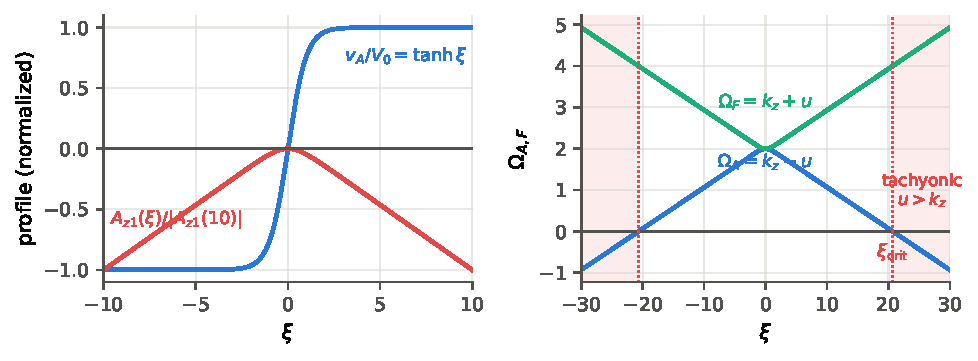
\includegraphics[width=\textwidth]{fig_background.pdf}
\caption{The production background. \emph{Left}: counter-streaming shear
$v_A=\Vo\tanh\xi$ (beam B is its mirror) and the frozen log-cosh potential
$\Az$ of eq.~\eqref{eq:Az1}, normalized to its value at $\xi=10$.
\emph{Right}: the covariant wavenumbers $\OmA=\kz-u$ and $\OmF=\kz+u$
(here $\alpha=2$, $\Vo=0.05$, $\kz=2$). Beyond
$\xi_{\mathrm{crit}}=\kz/(\alpha\Vo)+\ln2$ (dotted, shaded) the product
$\OmA\OmF$ is negative and one circular polarization is tachyonic
(\S\ref{sec:local}); inside, the same shift $u$ builds the confining well
of the shear branch (\S\ref{sec:reduction}).}
\label{fig:background}
\end{figure}

\subsection{Reading map}
Sections~\ref{sec:quartic}--\ref{sec:seeding} are ordered logically, not
chronologically: model $\to$ linearization $\to$ local theory $\to$ exact
reduction $\to$ drive/ceiling $\to$ quantization $\to$ dispersion-curve
consequences $\to$ scalings $\to$ nonlinear/auxiliary theory. Each section
states which numerical validation anchors it; the ledger is collected in
Appendix~\ref{app:ledger}. Indented \textcolor{intu}{\textbf{Physical
picture}} boxes carry the intuition behind each derivation. All figures
are generated from the formulas derived here by
\texttt{derivations/make\_figs.py}; the validation figure
(Fig.~\ref{fig:dispersion}) re-runs the repository's six-field eigensolver
rather than reusing cached curves.

% ==============================================================================
\section{From the harmonic-core quantization to the quartic, and the
$\kz=0$ chromo-Weibel rate}
\label{sec:quartic}

\subsection{Clearing eq.~(33) to a quartic polynomial}
\label{ssec:clearing}

\begin{step}
Substitute the definitions \eqref{eq:wkbQ}--\eqref{eq:wkbQ0} into
\eqref{eq:eq33}, with the background velocity scale written $v=\Vo$:
\begin{equation}
\omega^2-\kz^2-\frac{\alpha^2\Vo\kz}{\omega^2}
=(2n+1)\sqrt{\frac{\alpha^3\Vo^2}{2\,\omega^2}} .
\label{eq:eq33sub}
\end{equation}
\end{step}

\begin{step}
The square root on the right is resolved as
$\sqrt{\alpha^3/2}\,\Vo/\omega$. For real positive $\omega$ this is
elementary; for the complex (growing) roots we are about to find, this
choice of branch defines the analytic continuation used everywhere in the
program (the continuation is fixed by requiring the $\kz=0$ limit below to
reproduce the direct cubic factorization, which it does). Define the
constant
\begin{equation}
C\equiv(2n+1)\sqrt{\frac{\alpha^3}{2}}\;\Vo .
\label{eq:Cdef}
\end{equation}
Then \eqref{eq:eq33sub} reads
\begin{equation}
\omega^2-\kz^2-\frac{\alpha^2\Vo\kz}{\omega^2}=\frac{C}{\omega}.
\end{equation}
\end{step}

\begin{step}
Multiply through by $\omega^2$ (legitimate: $\omega=0$ is not a root of
\eqref{eq:eq33sub}) and collect all terms on one side:
\begin{equation}
\boxed{\;
\omega^4-\kz^2\,\omega^2-C\,\omega-\alpha^2\Vo\kz=0
\;}
\label{eq:quartic}
\end{equation}
This is the \emph{WKB quartic} (also \texttt{wkbfull.pdf} eq.~(4)); the
fastest-growing root $\gamma=\max\Imy\,\omega$ over its four roots is the
``$\gamma_{\mathrm{WKB}}$'' quoted in all program tables.
\end{step}

\begin{remark}[The growing root is not purely imaginary away from $\kz=0$]
\label{rem:notpureim}
An early implementation assumed $\Rey\,\omega=0$ and bisected on real
$\gamma$. Substituting $\omega=\ii\gamma$ into \eqref{eq:quartic} gives
$\gamma^4+\kz^2\gamma^2-\alpha^2\Vo\kz=\ii C\gamma$, whose left side is real
and right side imaginary --- so a purely imaginary root exists only where
$C\gamma$ can vanish, i.e.\ at $\kz=0$ (where the real part balances
differently, see below) or in the trivial limit $C\to0$. Numerically the
purely-imaginary assumption erred by up to $\sim50\%$ at $\kz=0.25$ and
$\sim10\%$ at $\kz=1$, shrinking with $\kz$; the full complex quartic is
solved everywhere in current tooling.
\end{remark}

\subsection{The $\kz=0$ limit: chromo-Weibel growth rate}
\label{ssec:weibel}

\begin{step}
Set $\kz=0$ in \eqref{eq:quartic}. Both the $\kz^2\omega^2$ term and the
constant term $\alpha^2\Vo\kz$ vanish:
\begin{equation}
\omega^4-C\omega=0
\qquad\Longleftrightarrow\qquad
\omega\,(\omega^3-C)=0 .
\end{equation}
\end{step}

\begin{step}
Discard the root $\omega=0$ (no dynamics). The cubic factor gives the three
cube roots of the positive real number $C$:
\begin{equation}
\omega\in\Bigl\{\,C^{1/3},\;
C^{1/3}e^{2\pi\ii/3},\;
C^{1/3}e^{-2\pi\ii/3}\Bigr\}.
\end{equation}
\end{step}

\begin{step}
The growing root is the one with positive imaginary part,
$\omega=C^{1/3}e^{2\pi\ii/3}$, with
\begin{equation}
\gamma=\Imy\,\omega
=C^{1/3}\sin\frac{2\pi}{3}
=\frac{\sqrt3}{2}\,C^{1/3}.
\end{equation}
\end{step}

\begin{step}
Insert $C$ from \eqref{eq:Cdef} for the fundamental $n=0$:
\begin{equation}
\boxed{\;
\gamma_{\mathrm{Weibel}}(\kz{=}0)
=\Bigl(\sqrt{\tfrac{\alpha^3}{2}}\;\Vo\Bigr)^{1/3}\,
\frac{\sqrt3}{2}
=\Bigl(\sqrt{\tfrac{\alpha^3}{2}}\;\Vo\Bigr)^{1/3}\sin 60^\circ
\;}
\label{eq:weibel}
\end{equation}
\end{step}

\begin{remark}[Physical content and validation]
At $\kz=0$ the unstable channel is a color-mixing filamentation
(``chromo-Weibel'') mode: the background $\Az$ mixes the color-2 and
color-3 electromagnetic fields through the non-Abelian Amp\`ere term
$-\alpha(A_z\times B_y)^a$ and Faraday term $+\alpha(A_z\times E_x)^a$
(\S\ref{sec:model}), producing $z$-uniform exponentially growing color-2/3
fields. Direct simulation reproduced \eqref{eq:weibel} to $0.5\%$, the
strongest single anchor of the quartic. This mode is deliberately
suppressed in production KH campaigns (\texttt{suppress\_kz0=1} plus
hyperdiffusion, Appendix~\ref{app:filters}); at the reference point of the
self-consistency study (\S\ref{ssec:backreaction}), $\alpha=1$, $\Vo=0.05$,
formula \eqref{eq:weibel} gives $\gamma=0.284$, exactly the measured
irreducible $\kz=0$ growth there. Figure~\ref{fig:quartic} shows the
quartic's dispersion curves with the $\kz=0$ anchors.
\end{remark}

\begin{intuition}
At $\kz=0$ nothing varies along the flow, so this is not a bunching
instability but \emph{filamentation}: the frozen $\Az$ rotates the
color-2/3 fields into each other while the counter-streaming color
currents feed them, and the displaced currents reinforce the seed field.
The cube root in \eqref{eq:weibel} is the signature of the loop: closing
the feedback ($E\to A$ by one time integration, $A\to Q$ by a second,
$Q\to J\to E$ by a third) gives a loop gain $\propto C/\gamma^3$; marginal
self-amplification, gain of order one, fixes $\gamma\sim C^{1/3}$, and the
exact root geometry supplies the $\sin 60^\circ$.
\end{intuition}

\begin{figure}[t]
\centering
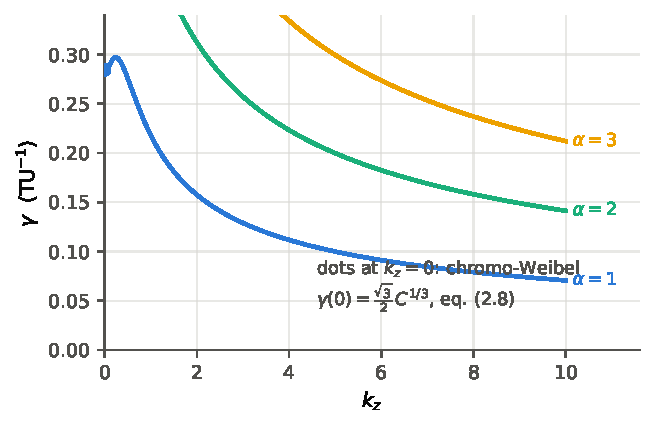
\includegraphics[width=0.62\textwidth]{fig_quartic.pdf}
\caption{The WKB quartic \eqref{eq:quartic} at $\Vo=0.05$ for
$\alpha=1,2,3$ ($n=0$), with the exact $\kz=0$ chromo-Weibel roots
\eqref{eq:weibel} (dots). The $\kz=0$ anchor is validated to $0.5\%$ in
simulation; the finite-$\kz$ behaviour of the quartic is its
harmonic-core extrapolation, superseded by the exact-action theory ---
see the diagnosis in \S\ref{sec:gap} and the direct comparison in
Fig.~\ref{fig:dispersion}.}
\label{fig:quartic}
\end{figure}

% ==============================================================================
\section{The time-domain model as posed}
\label{sec:model}

The nonlinear system integrated by the CUDA code is the time-domain
counterpart of the linearized system of \texttt{khaxn.pdf}. It is stated
here as the model definition; the derivations in this section are (i) the
Wong-equation origin of the precession source, (ii) the invariant
$B_y^a=-\partial_xA_z^a$ of the potential/Faraday pair, and (iii) the exact
energy budget, which identifies the frozen background as an external
battery.

\subsection{Model equations}
\label{ssec:modeleqs}

Fields: for each color $a\in\{1,2,3\}$, the 2D $(x,z)$ fields $E_x^a$,
$E_z^a$, $B_y^a$, $A_z^a$; for each beam $s\in\{A,B\}$, the fluid fields
$n_s$, $p_{xs}$, $p_{zs}$ (momentum densities; $v_{is}=p_{is}/n_s$) and the
color-charge densities $Q^a_s$. Only $A_z^a$ is carried as an explicit
potential ($\partial_y\equiv0$; no $y$-components of $E$ or of the fluid
velocity are excited by the dynamics below). The gauge choice this
reflects, and the precise (non-)status of $A_x^a$ and $A_y^a$, is examined
in \S\ref{ssec:gaugecount} immediately below: in short, $A_0^a\equiv0$ is
the one legitimate gauge condition spent here, while the absence of
$A_y^a$ and $A_x^a$ are two separate statements of a different kind, not a
second gauge-fixing.

\paragraph{Fluid sector} (each beam; FCT advection):
\begin{align}
&\partial_t n+\nabla\!\cdot\!(n\vec v)=0,
\label{eq:continuity}\\
&\partial_t p_x+\nabla\!\cdot\!(\vec v\,p_x)=F_x
=-n\sum_a Q^a\bigl(E_x^a+v_zB_y^a\bigr),
\label{eq:momx}\\
&\partial_t p_z+\nabla\!\cdot\!(\vec v\,p_z)=F_z
=-n\sum_a Q^a\bigl(E_z^a-v_xB_y^a\bigr),
\label{eq:momz}\\
&\partial_t Q^a+\nabla\!\cdot\!(\vec v\,Q^a)
=\alpha\,v_z\,(\vec Q\times\vec A_z)^a ,
\label{eq:precession}
\end{align}
where $(\vec Q\times \vec A_z)^a=\epsilon^{abc}Q^bA_z^c$ is the SU(2)
adjoint cross product. (In \eqref{eq:precession} the $Q^a$ are advected as
densities; combined with \eqref{eq:continuity} this is equivalent to the
advective form $\dd Q^a/\dd t=\alpha v_z(\vec Q\times\vec A_z)^a$ along
fluid trajectories, which is what Wong's equation supplies,
\S\ref{ssec:wong}.)

\paragraph{Field sector} (leapfrog on a Yee stagger):
\begin{align}
&\partial_t E_x^a=-\partial_z B_y^a-\alpha\,(\vec A_z\times\vec B_y)^a
-J_x^a ,
\label{eq:amperex}\\
&\partial_t E_z^a=+\partial_x B_y^a-J_z^a ,
\label{eq:amperez}\\
&\partial_t B_y^a=\partial_x E_z^a-\partial_z E_x^a
+\alpha\,(\vec A_z\times\vec E_x)^a ,
\label{eq:faraday}\\
&\partial_t A_z^a=-E_z^a
\qquad(\text{$A_z^1$ held fixed when \texttt{freeze\_az1}=1}),
\label{eq:potential}\\
&J_i^a=-\,n_AQ^a_Av_{iA}-n_BQ^a_Bv_{iB},\qquad i\in\{x,z\} .
\label{eq:currents}
\end{align}
Equation \eqref{eq:amperez} carries no non-Abelian term: the candidate
commutator $\alpha\epsilon^{abc}A_z^bF^{zz,c}$ vanishes identically because
only the $z$-component of the potential is kept. The sign conventions
(charge enters the current and the force with an overall minus) are the
model's own; their only invariant consequences are the products
current$\times$field and force$\times$velocity, and those are fixed by the
energy budget below.

\subsection{Gauge counting: what the field content assumes}
\label{ssec:gaugecount}

The field content just declared silently makes a claim worth checking
explicitly: that dropping $A_x^a$ and $A_y^a$ while keeping only $A_z^a$
is licensed by gauge freedom. It is not, quite --- the SU(2) gauge group
supplies exactly enough freedom to eliminate \emph{one} full
spacetime-component of $A_\mu^a$, not two, and the argument for why the
model is nonetheless consistent has two genuinely different parts.

\begin{step}[The counting]
An infinitesimal SU(2) gauge transformation is parametrized by
$\theta^a(t,x,z)$, $a=1,2,3$: three arbitrary functions of the three
coordinates the fields depend on here ($\partial_y\equiv0$ removes $y$
from the list), transforming $\delta A_\mu^a=-(D_\mu\theta)^a$. A
condition such as ``$A_x^a(t,x,z)=0$ for all $(t,x,z)$'' is three
equations (one per color) holding at every point of a three-dimensional
domain --- exactly as many conditions as gauge functions available.
Generically this exhausts the freedom (up to a residual gauge
transformation independent of $x$, the integration freedom left when
solving $\partial_x\theta^a=(\cdots)$ pointwise in $x$). The general
statement:
\begin{equation}
\boxed{\text{one gauge choice}\;\Longrightarrow\;\text{one full
spacetime component of }A_\mu^a\text{ eliminated --- not two.}}
\label{eq:gaugecounting}
\end{equation}
\end{step}

\begin{step}[What \texttt{khaxn.pdf} spends its one choice on]
Its stated gauge is $a_x^a=0$, and nothing else. In particular:
\begin{itemize}
\item $\phi\equiv A_0$ is \emph{not} set to zero. It survives as a
genuine background field ($E^1_{0x}=-\partial_x\phi^1_0$, its \S1) and
perturbation field, eliminated only via the Gauss-law \emph{constraint}
--- a fundamentally different move from a gauge choice --- in its own
``Substitution and Simplification'' section, solving $\phi^+$ in terms of
$a_z^+$.
\item $a_y^a$ is not set to zero either: it is explicitly retained and
sources $b_x$ (its eq.~1). Its own ``Final equations'' \S2 shows
$a_y^\pm$ (eq.~22) and $a_z^+$ with $\phi$ eliminated (eq.~23) form two
separate equations, not interacting with each other at this order.
\end{itemize}
The surviving content after \texttt{khaxn.pdf}'s one gauge choice is
therefore $(\phi,a_y,a_z)$, not $a_z$ alone.
\end{step}

\begin{step}[What the simulated model spends its one choice on]
The potential equation \eqref{eq:potential}, $\partial_tA_z^a=-E_z^a$, is
the exact temporal-gauge relation $E_z=-\partial_tA_z$ with no
$-\partial_zA_0$ correction term. This identifies the model's one gauge
condition as
\begin{equation}
A_0^a\equiv0 \qquad\text{(temporal gauge)},
\end{equation}
a legitimate, complete choice --- and a \emph{different} one from
\texttt{khaxn.pdf}'s axial choice, not an additional condition stacked on
top of it.
\end{step}

\begin{step}[Why $A_y^a$ and $A_x^a$ can then be dropped without spending
more freedom]
Two separate arguments, of two different kinds:
\begin{itemize}
\item \emph{$A_y^a$ is a sector choice, not a gauge choice.} The
$a_y^\pm$ branch (\texttt{khaxn.pdf} eq.~22) does not source, or get
sourced by, the $a_z$ branch; the perturbation studied here (By2-type
seeding, \S\ref{sec:seeding}) never populates it. Omitting it selects
\emph{which already-decoupled physical sector to simulate} --- licensed
by the decoupling \texttt{khaxn.pdf} itself exhibits, not by spending
extra gauge freedom. (Restated as the scope remark of
\S\ref{ssec:scope}.)
\item \emph{$A_x^a$ is wired to nothing.} Unlike $A_y^a$, this field
does not merely go unsourced by the chosen initial data --- it never
appears, at all, in any covariant or commutator term of
eqs.~\eqref{eq:momx}--\eqref{eq:currents}: every non-Abelian correction
in the model (Amp\`ere-$x$, Faraday, precession) references $\vec A_z$
only. A hypothetical $A_x^a$ generated by some other mechanism would
still have zero effect on any other field's equation of motion; it is a
complete spectator, consistently left untracked regardless of its own
value.
\end{itemize}
\end{step}

\begin{intuition}
One knob, one turn. Gauge freedom is a redundancy in the description,
not in the physics: the count of gauge functions must match the count of
unphysical directions removed. \texttt{khaxn.pdf} turns the ``$A_x$''
knob and leaves $\phi$, $a_y$ as real content --- one eliminated by a
constraint, the other by non-interaction with the sector of interest.
This model turns a \emph{different} knob, ``$A_0$'' --- equally
legitimate, equally a single turn --- and then drops $A_y$ for a
decoupling reason and $A_x$ because it is wired to nothing. Two
different single choices of gauge are not the same thing as one gauge
choice spent twice.
\end{intuition}

\begin{remark}[Consistency check: $E_x$ is not spurious content]
If the model had silently fixed both $A_x=0$ and $A_0=0$, its would-be
substitute for $\phi$ --- namely $E_x$ --- ought to carry independent new
physics absent from \texttt{khaxn.pdf}'s construction. It does not: the
linearized Amp\`ere-$x$ equation derived in \S\ref{sec:sixfield},
eq.~\eqref{eq:lin-ex} ($\gamma e_x=-\ii\OmA b$), shows $e_x$ is purely
and instantaneously slaved to $b$ --- a first-order algebraic relation,
not an independently propagating mode. This is exactly the behavior a
properly constraint-eliminated $\phi$ must have: $E_x$ here plays
$\phi$'s role in temporal-gauge dress, rather than adding unphysical
content the given theory does not have.
\end{remark}

\subsection{Derivation of the precession source from Wong's equations}
\label{ssec:wong}

\begin{step}
Wong's equation for the color charge of a classical particle moving on a
worldline $x^\mu(\tau)$ in a background potential $A^b_\mu$ is
\begin{equation}
\frac{\dd Q^a}{\dd\tau}
+g\,\epsilon^{abc}\,\frac{\dd x^\mu}{\dd\tau}A^b_\mu\,Q^c=0 .
\end{equation}
\end{step}

\begin{step}
Non-relativistic limit ($\tau\to t$, $\dd x^\mu/\dd\tau\to(1,\vec v)$),
temporal gauge $A^b_0=0$, and only $A^b_z\neq0$:
\begin{equation}
\frac{\dd Q^a}{\dd t}
=-g\,\epsilon^{abc}\,v_zA_z^b\,Q^c .
\end{equation}
\end{step}

\begin{step}
Rename $g\to\alpha$ and swap the summed indices $b\leftrightarrow c$ using
antisymmetry, $\epsilon^{abc}A^bQ^c=-\epsilon^{abc}Q^bA^c$:
\begin{equation}
\frac{\dd Q^a}{\dd t}
=+\alpha\,v_z\,\epsilon^{abc}Q^bA_z^c
=\alpha\,v_z\,(\vec Q\times\vec A_z)^a ,
\end{equation}
which is exactly the source in \eqref{eq:precession}. Because $|\vec Q|$ is
conserved by a cross-product rotation, $Q^1_{A,B}=\pm1$ remains a unit
adjoint vector until advection mixes fluid elements.
\end{step}

\subsection{The invariant $B_y^a=-\partial_xA_z^a$ of the potential pair}
\label{ssec:byinvariant}

From \eqref{eq:potential}, $\partial_t(-\partial_xA_z^a)=\partial_xE_z^a$.
Comparing with \eqref{eq:faraday}, the difference field
$W^a\equiv B_y^a+\partial_xA_z^a$ obeys
\begin{equation}
\partial_t W^a=-\partial_zE_x^a+\alpha(\vec A_z\times\vec E_x)^a .
\label{eq:Wevol}
\end{equation}
Thus $B_y=-\partial_xA_z$ (the magnetostatic relation, matching
\texttt{khaxn.pdf} eqs.~(4)--(6), $b_y^a=-\partial_xa_z^a$) is preserved
exactly for $z$-uniform, color-aligned configurations
(e.g.\ the color-1 background itself, for which the right side of
\eqref{eq:Wevol} vanishes), but \emph{not} for the color-2/3 wave sector,
where $B_y$ carries the additional dynamics injected through $E_x$. This is
why the code treats $B_y^a$ as an independent evolved field, and why a
current-consistent $B_{y1}$ initialization (\texttt{init\_by1\_eq}) is
needed when the color-1 sector is live (\S\ref{ssec:backreaction}).

\subsection{Exact energy budget: conservative core plus the frozen-background
battery}
\label{ssec:energy}

The monitored energy is
\begin{equation}
E(t)=\int\!\dd x\,\dd z\;\Bigl[
\tfrac12\sum_a\bigl((E_x^a)^2+(E_z^a)^2+(B_y^a)^2\bigr)
+\sum_{s=A,B}\frac{p_{xs}^2+p_{zs}^2}{2n_s}\Bigr].
\label{eq:energydef}
\end{equation}
We differentiate term by term using
\eqref{eq:continuity}--\eqref{eq:currents}, at the continuum level and over
the periodic box (so all pure divergences integrate to zero).

\begin{step}[Setting up the calculation]
Differentiate \eqref{eq:energydef} under the integral sign. The field part
is immediate from the product rule,
\begin{equation}
\frac{\dd}{\dd t}\Bigl[\tfrac12\sum_a\bigl((E_x^a)^2+(E_z^a)^2+(B_y^a)^2\bigr)\Bigr]
=\sum_a\Bigl[E_x^a\,\partial_tE_x^a+E_z^a\,\partial_tE_z^a+B_y^a\,\partial_tB_y^a\Bigr],
\end{equation}
and each $\partial_t(\cdot)$ is then replaced by the \emph{full}
right-hand side of \eqref{eq:amperex}--\eqref{eq:faraday} --- curl term,
current term, and non-Abelian commutator term alike; nothing is dropped at
this stage, and the three steps below simply sort the resulting terms into
three physically distinct piles.

The fluid part needs one extra piece of algebra because $n_s$ also depends
on $t$. Write $K_i\equiv p_i^2/(2n)$ for either momentum component of
either beam (beam label suppressed) and use the chain rule together with
\eqref{eq:continuity}--\eqref{eq:momz}:
\begin{equation}
\partial_tK_i=\frac{p_i}{n}\,\partial_tp_i-\frac{p_i^2}{2n^2}\,\partial_tn
=v_i\bigl[-\nabla\!\cdot\!(\vec v\,p_i)+F_i\bigr]
-\frac{v_i^2}{2}\bigl[-\nabla\!\cdot\!(n\vec v)\bigr].
\end{equation}
Expand both divergences with the product rule, using $p_i=nv_i$:
$\nabla\!\cdot\!(\vec v\,p_i)=v_i\nabla\!\cdot\!(n\vec v)
+n\,\vec v\!\cdot\!\nabla v_i$. Substituting and collecting the two
$\nabla\!\cdot\!(n\vec v)$ pieces (coefficients $-v_i^2$ and $+v_i^2/2$,
net $-v_i^2/2$):
\begin{equation}
\partial_tK_i=-\tfrac12v_i^2\,\nabla\!\cdot\!(n\vec v)
-n v_i(\vec v\!\cdot\!\nabla v_i)+v_iF_i .
\end{equation}
Compare with $\nabla\!\cdot\!(\vec vK_i)=\nabla\!\cdot\!\bigl(\vec v\,
nv_i^2/2\bigr)=\tfrac12v_i^2\,\nabla\!\cdot\!(n\vec v)
+nv_i(\vec v\!\cdot\!\nabla v_i)$ (same product rule, run on $K_i$
directly): the right side above is exactly $-\nabla\!\cdot\!(\vec vK_i)$
plus the leftover $v_iF_i$. Hence the fluid kinetic-energy identity used
below,
\begin{equation}
\partial_tK_i=-\nabla\!\cdot\!(\vec v\,K_i)+v_iF_i ,
\label{eq:kinlemma}
\end{equation}
holding term by term for $i\in\{x,z\}$ and each beam: transport is
conservative (a pure divergence, integrates to zero over the periodic box),
and the only source is $v_iF_i$ --- structurally identical to the field
energy, where transport is the Poynting divergence and the only source is
the work $\vec J\cdot\vec E$ plus the non-Abelian terms.
\end{step}

\begin{step}[Transport terms]
The Maxwell curl terms combine into divergences:
\begin{equation}
E_x^a(-\partial_zB_y^a)+B_y^a(-\partial_zE_x^a)=-\partial_z(E_x^aB_y^a),
\qquad
E_z^a(\partial_xB_y^a)+B_y^a(\partial_xE_z^a)=\partial_x(E_z^aB_y^a),
\end{equation}
i.e.\ a Poynting flux; both integrate to zero. Likewise, for smooth flow
the FCT advection terms transport $\tfrac12p^2/n$ conservatively:
using \eqref{eq:continuity}--\eqref{eq:momz} without sources,
$\partial_t(p_i^2/2n)+\nabla\!\cdot(\vec v\,p_i^2/2n)=0$.
\end{step}

\begin{step}[Current work cancels against the Lorentz work]
The field sector loses $\sum_a(J_x^aE_x^a+J_z^aE_z^a)=\vec J^a\!\cdot\vec
E^a$; with \eqref{eq:currents} this equals
$-\sum_s n_s\sum_aQ_s^a\,\vec v_s\!\cdot\vec E^a$. The fluid sector gains
$\sum_s\vec v_s\cdot\vec F_s$ with $\vec F_s$ from
\eqref{eq:momx}--\eqref{eq:momz}; the magnetic parts cancel within the dot
product,
\begin{equation}
v_x(v_zB_y^a)+v_z(-v_xB_y^a)=0,
\end{equation}
leaving $\sum_s\vec v_s\cdot\vec F_s
=-\sum_sn_s\sum_aQ^a_s\,\vec v_s\!\cdot\!\vec E^a$. The two contributions are
equal and opposite: energy flows between fields and fluid with no loss.
(This is the invariant content of the model's charge-sign convention: the
same minus sign appears in \eqref{eq:currents} and in
\eqref{eq:momx}--\eqref{eq:momz}, so all work terms pair correctly.)
\end{step}

\begin{step}[Non-Abelian cross terms: the battery]
Collect what is left after the previous two steps. Substitute the full
right-hand sides of \eqref{eq:amperex} and \eqref{eq:faraday} into the
field part of $\dd E/\dd t$ set up above, and the full
\eqref{eq:momx}--\eqref{eq:momz} into the fluid part via
\eqref{eq:kinlemma}. Every term is now accounted for except two: the
commutator piece of Amp\`ere-$x$, multiplied by $E_x^a$, and the
commutator piece of Faraday, multiplied by $B_y^a$ (the curl pieces became
the Poynting flux of the transport step and integrate to zero; the current
pieces cancelled against the Lorentz-force work of the previous step; the
fluid transport pieces of \eqref{eq:kinlemma} also integrate to zero, same
step). What remains is
\begin{equation}
\frac{\dd E}{\dd t}\bigg|_{\mathrm{NA}}
=\int\Bigl[\underbrace{E_x^a\cdot\bigl(-\alpha(\vec A_z\times\vec B_y)^a\bigr)}
_{\text{leftover from Amp\`ere-}x}
+\underbrace{B_y^a\cdot\bigl(+\alpha(\vec A_z\times\vec E_x)^a\bigr)}
_{\text{leftover from Faraday}}\Bigr],
\end{equation}
i.e., writing out the two commutators (sum over the repeated color index
$a$ understood in each product),
\begin{equation}
\frac{\dd E}{\dd t}\bigg|_{\mathrm{NA}}
=\int\Bigl[-\alpha\sum_a E_x^a(\vec A_z\times\vec B_y)^a
+\alpha\sum_a B_y^a(\vec A_z\times\vec E_x)^a\Bigr].
\end{equation}
\end{step}

\begin{step}[An epsilon-tensor identity]
Write both terms as scalar triple products in color space,
$[\vec X,\vec Y,\vec Z]\equiv\epsilon^{abc}X^aY^bZ^c$ (sum over
$a,b,c\in\{1,2,3\}$; the first vector supplies the free index that is also
the $\epsilon$ tensor's first slot), so
$\sum_aE_x^a(\vec A_z\times\vec B_y)^a=[\vec E_x,\vec A_z,\vec B_y]$ and
$\sum_aB_y^a(\vec A_z\times\vec E_x)^a=[\vec B_y,\vec A_z,\vec E_x]$. We need
the relation between these two. Start from the second and relabel the three
\emph{dummy} summation indices $a\to c,\,b\to b,\,c\to a$ (legal: summed
indices carry no meaning of their own):
\begin{equation}
[\vec B_y,\vec A_z,\vec E_x]=\epsilon^{abc}B_y^aA_z^bE_x^c
=\epsilon^{cba}B_y^cA_z^bE_x^a
=\epsilon^{cba}\,E_x^aA_z^bB_y^c .
\end{equation}
The index string $\epsilon^{cba}$ differs from $\epsilon^{abc}$ only by
swapping the 1st and 3rd slots ($a\leftrightarrow c$) --- a single
transposition, which flips the sign of the totally antisymmetric symbol:
$\epsilon^{cba}=-\epsilon^{abc}$ (spot check: $\epsilon^{213}=-\epsilon^{123}
=-1$, consistent with the definition $\epsilon^{123}=+1$ and total
antisymmetry). Hence
\begin{equation}
[\vec B_y,\vec A_z,\vec E_x]=-\epsilon^{abc}E_x^aA_z^bB_y^c
=-[\vec E_x,\vec A_z,\vec B_y].
\label{eq:tripleflip}
\end{equation}
In words: swapping the outer two vectors of a triple product costs a minus
sign, with the middle vector as a spectator. This is the general rule
behind every ``$[\cdots]=-[\cdots]$'' step used in the program.
\end{step}

\begin{step}[Assembling the battery term]
Insert \eqref{eq:tripleflip} into the result of the first step of this
sequence:
\begin{align}
\frac{\dd E}{\dd t}\bigg|_{\mathrm{NA}}
&=-\alpha\int[\vec E_x,\vec A_z,\vec B_y]
+\alpha\int[\vec B_y,\vec A_z,\vec E_x]\notag\\
&=-\alpha\int[\vec E_x,\vec A_z,\vec B_y]-\alpha\int[\vec E_x,\vec A_z,\vec B_y]
=-2\alpha\int[\vec E_x,\vec A_z,\vec B_y] .
\end{align}
Finally translate back to an ordinary dot-and-cross product:
$[\vec E_x,\vec A_z,\vec B_y]=\vec A_z\cdot(\vec B_y\times\vec E_x)$. Proof:
in components, $(\vec B_y\times\vec E_x)^b=\epsilon^{bca}B_y^cE_x^a$ (the
standard formula, indices cycled), so
\begin{equation}
\vec A_z\cdot(\vec B_y\times\vec E_x)
=A_z^b\,\epsilon^{bca}B_y^cE_x^a
=\epsilon^{bca}E_x^aA_z^bB_y^c .
\end{equation}
The index string $bca$ is a \emph{cyclic} permutation of $abc$
($a\to b\to c\to a$), and cyclic permutations of $\epsilon$ are always even
(no sign change: two transpositions), so $\epsilon^{bca}=\epsilon^{abc}$,
and the two expressions agree term by term:
$\vec A_z\cdot(\vec B_y\times\vec E_x)=\epsilon^{abc}E_x^aA_z^bB_y^c
=[\vec E_x,\vec A_z,\vec B_y]$. Therefore
\begin{equation}
\frac{\dd E}{\dd t}\bigg|_{\mathrm{NA}}
=-2\alpha\int \vec A_z\cdot(\vec B_y\times\vec E_x).
\label{eq:battery}
\end{equation}
This does \emph{not} vanish in general: the model's quadratic energy
\eqref{eq:energydef} is not the full Yang--Mills energy (which hides the
interaction energy inside the field-strength commutators), and
\eqref{eq:battery} is precisely the exchange with the potential sector.
\end{step}

\begin{step}[Evaluation on the frozen background]
Unlike $\vec A_z$, whose color-2/3 components really are pure wave
perturbation (absent from the background, \S\ref{sec:sixfield}), $\vec B_y$
and $\vec E_x$ each already have a nonzero color-1 \emph{background} piece
in general --- this is not automatic and must be checked separately for
each, since neither is protected by the same ``wave-only'' argument that
lets $\vec A_z\approx(\Az,a_2,a_3)$ with only $a_2,a_3$ small.
\begin{itemize}
\item $E_x^1$: in steady state, its source in Amp\`ere-$x$
\eqref{eq:amperex} is $-\partial_zB_y^1-\alpha(\vec A_z\times\vec B_y)^1
-J_x^1$. The background is $z$-independent (kills the curl term); the
commutator $(\vec A_z\times\vec B_y)^1=A_z^2B_y^3-A_z^3B_y^2$ needs a
background $A_z^{2,3}$, which is zero; and $J_x^1=0$ since neither beam
carries background $v_x$ \eqref{eq:beams}. So $E_x^1$ has no background
source at all, and (matching the code's initialization) $E_x^1\equiv0$ in
the background is exact, not an approximation.
\item $B_y^1$: by contrast, the invariant of \S\ref{ssec:byinvariant},
$B_y^a=-\partial_xA_z^a$, applies to the $z$-uniform color-1 background
exactly, so $B_y^1=-\partial_x\Az(\xi)\not\equiv0$ whenever $\Az$ has
$x$-structure --- which it always does (it is the shear-coupling
background). This is a genuine, nonzero background field, consistent
with the code's own gauge-consistent initialization of \texttt{By1}.
\end{itemize}
Expand the full dot product $\vec A_z\cdot(\vec B_y\times\vec E_x)
=\sum_b A_z^b(\vec B_y\times\vec E_x)^b$ term by term in $b$, using
$\vec A_z=(\Az,a_2,a_3)$, $\vec B_y=(B_y^1,B_y^2,B_y^3)$,
$\vec E_x=(0,E_x^2,E_x^3)$ (the just-established $E_x^1=0$):
the $b{=}1$ term gives $\Az(B_y^2E_x^3-B_y^3E_x^2)$ exactly as before; the
$b{=}2,3$ terms, worked out the same way as \eqref{eq:crosscomponents}--%
\eqref{eq:crosscomplex} but now with $E_x^1=0$, collapse to
$B_y^1(a_3E_x^2-a_2E_x^3)=B_y^1\,\Imy(a\,e_x^*)$ (circular pairs
$a=a_2+\ii a_3$, $e_x=E_x^2+\ii E_x^3$; check by direct expansion:
$a\,e_x^*=(a_2+\ii a_3)(E_x^2-\ii E_x^3)$ has imaginary part
$a_3E_x^2-a_2E_x^3$). So, exactly,
\begin{equation}
\vec A_z\cdot(\vec B_y\times\vec E_x)
=\Az\,\bigl(B_y^2E_x^3-B_y^3E_x^2\bigr)+B_y^1\,\Imy(a\,e_x^*).
\label{eq:battery-full}
\end{equation}
The second term is the same order in the wave amplitude as the first: both
are one factor of background times two factors of wave. It is \emph{not}
generally negligible on formal grounds. In the production geometry
(mode 5, \S\ref{sec:sixfield}) it happens to be small, but for a reason
specific to that background's geometry, not a perturbative smallness.
$\Az=-\Vo\cos(k_xx)$ is engineered to peak, flat to second order, exactly
at the shear layer where the KH eigenfunction is supported. Its derivative
$B_y^1=-\Vo k_x\sin(k_xx)$ vanishes there and grows only linearly with
distance from the layer, over that same support. So the two factors in the
second term are small together, in the one region that matters, even
though $B_y^1$'s
\emph{global} maximum (far from the layer, where the eigenfunction has
already decayed) is not small. This is the same omission already flagged,
and bounded empirically at the few-percent level against the full
simulation, in the six-field system's scope remark
(\S\ref{ssec:scope}, item 2); it is not re-derived here, and the rest of
this step keeps only the leading (first) term, so every result downstream
of \eqref{eq:batterysign} inherits this few-percent-level caveat.

Substituting the leading term into \eqref{eq:battery}:
\begin{equation}
\frac{\dd E}{\dd t}\bigg|_{\mathrm{NA}}
=-2\alpha\int \Az\,\bigl(B_y^2E_x^3-B_y^3E_x^2\bigr).
\end{equation}
Now introduce the same complex ``circular'' pairs used throughout
\S\ref{sec:sixfield}, $b=B_y^2+\ii B_y^3$ and $e_x=E_x^2+\ii E_x^3$ --- at
this point purely a notational bundling of two real numbers into one
complex one, nothing physical yet. Multiply out
\begin{equation}
b^{*}e_x=(B_y^2-\ii B_y^3)(E_x^2+\ii E_x^3)
=\underbrace{\bigl(B_y^2E_x^2+B_y^3E_x^3\bigr)}_{\Rey(b^*e_x)}
+\ii\underbrace{\bigl(B_y^2E_x^3-B_y^3E_x^2\bigr)}_{\Imy(b^*e_x)},
\end{equation}
so the bracket above is exactly $\Imy(b^*e_x)$:
\begin{equation}
\frac{\dd E}{\dd t}\bigg|_{\mathrm{NA}}
=-2\alpha\int\Az\;\Imy\!\left(b^{*}e_x\right).
\label{eq:battery23}
\end{equation}
Now use the linearized Amp\`ere-$x$ relation derived independently in
\S\ref{sec:sixfield}, $\gamma e_x=-\ii\OmA b$ (eq.~\eqref{eq:lin-ex} below)
--- legitimate here because it is simply the statement that $e_x$ and $b$
are not independent once the equations of motion hold. Solve for
$e_x=-\ii\OmA b/\gamma$ (real $\gamma$, $\OmA$ for a mode on the
real-$\gamma$ branch) and substitute:
\begin{align}
b^*e_x&=b^*\Bigl(\frac{-\ii\OmA b}{\gamma}\Bigr)
=\frac{-\ii\OmA}{\gamma}\,b^*b\notag\\
&=\frac{-\ii\OmA}{\gamma}\,|b|^2,
\end{align}
using $b^*b=|b|^2$ (real, non-negative). A number of the form
$-\ii\times(\text{real})$ has $\Imy=-(\text{that real number})$, so
$\Imy(b^*e_x)=-(\OmA/\gamma)|b|^2$. Substituting back into
\eqref{eq:battery23}:
\begin{equation}
\frac{\dd E}{\dd t}\bigg|_{\mathrm{NA}}
=-2\alpha\int\Az\Bigl(-\frac{\OmA}{\gamma}|b|^2\Bigr)
=\frac{2\alpha}{\gamma}\int\Az\,\OmA\,|b|^2 .
\label{eq:batterysign}
\end{equation}
In the tachyonic outer region (\S\ref{sec:local}) $\OmA=\kz-u<0$ while
$\Az<0$: the integrand is positive --- the frozen background \emph{feeds}
the wave, and with \texttt{freeze\_az1}=1 the battery is bottomless. In the
shear-branch well $\OmA>0$ and the same term is an energy drain; the shear
branch instead grows at the expense of the beams' kinetic energy through the
(internally cancelling) current-work channel. Equation
\eqref{eq:batterysign} is the energetic statement of the freeze artifact
discussed in \S\ref{ssec:tachyon} and measured in \S\ref{ssec:backreaction}.
\end{step}

\begin{intuition}
A frozen field is an infinite battery. Holding $\Az$ fixed is the
field-theory analogue of an external magnet held in place by an
unmodelled agent: any process that extracts energy from it can run
forever, and \eqref{eq:battery} is the wire through which the charge
flows. The tachyonic branch of \S\ref{sec:local} is precisely the
discharge of this battery into charged waves --- the 2D analogue of the
decay of a constant chromomagnetic background (Nielsen--Olesen). The
shear branch draws on a different account, the beams' bulk kinetic
energy, which is a legitimate, self-consistently modelled reservoir ---
which is why windowing away the battery-powered branch while keeping the
flow-powered one is a physically meaningful excision and not a fudge.
\end{intuition}

\begin{remark}[Covariant Gauss constraint]
The monitored (not enforced) constraint is the covariant Gauss law
$\partial_xE_x^a+\partial_zE_z^a+\alpha\epsilon^{abc}A_z^bE_z^c=\rho^a$ with
$\rho^a=-\sum_sn_sQ^a_s$, checked numerically by \texttt{gauss\_check.py};
the leapfrog scheme preserves it to discretization accuracy in the same way
the standard Yee scheme preserves the Abelian constraint.
\end{remark}
% ==============================================================================
\section{Linearization: the six-field circular system}
\label{sec:sixfield}

This section derives, in full detail, the linear eigenvalue system
implemented by the 1D solver \texttt{ym\_eigenmode.py} and reduced by all
later theory. It was validated against the 2D simulation at the
$1$--$4\%$ level across the production grid.

\subsection{Background and perturbation ansatz}

Background (mode 1/6 geometry): beams \eqref{eq:beams}, frozen potential
\eqref{eq:Az1}, all other fields zero. Write $v(\xi)\equiv\Vo\tanh\xi$ so
$v_{zA}=v$, $v_{zB}=-v$. Perturbations of the color-2/3 sector are combined
into complex ``circular'' pairs
\begin{equation}
b=B_y^2+\ii B_y^3,\quad
e_x=E_x^2+\ii E_x^3,\quad
e_z=E_z^2+\ii E_z^3,\quad
a=A_z^2+\ii A_z^3,\quad
q_{A,B}=Q^2_{A,B}+\ii Q^3_{A,B},
\label{eq:circpairs}
\end{equation}
each with the ansatz $f(x,z,t)=\hat f(x)\,e^{\ii\kz z+\gamma t}$, i.e.
\begin{equation}
\partial_t\to\gamma,\qquad \partial_z\to\ii\kz .
\end{equation}
Why circular pairs work: every non-Abelian term in
\eqref{eq:amperex}--\eqref{eq:potential} and \eqref{eq:precession} is a
cross product with the color-1 background, and this always reduces to a
single phase multiplication. Recall the general cross-product component
formula $(\vec Y\times\vec X)^i=\epsilon^{ijk}Y^jX^k$, i.e.\
$(\vec Y\times\vec X)^1=Y^2X^3-Y^3X^2$,
$(\vec Y\times\vec X)^2=Y^3X^1-Y^1X^3$,
$(\vec Y\times\vec X)^3=Y^1X^2-Y^2X^1$. Apply this with $\vec Y=\vec A_z
=(\Az,0,0)$ (only $Y^1=\Az$ nonzero) and a generic color vector
$\vec X=(X^1,X^2,X^3)$ whose own color-1 component $X^1$ is either absent
(the perturbed color-2/3 fields have no color-1 part by definition) or
decoupled at this order (see the parenthetical below):
\begin{align}
(\vec A_z\times\vec X)^2&=Y^3X^1-Y^1X^3=0-\Az X^3=-\Az X^3,\\
(\vec A_z\times\vec X)^3&=Y^1X^2-Y^2X^1=\Az X^2-0=+\Az X^2 .
\label{eq:crosscomponents}
\end{align}
Combine these as $(2)+\ii(3)$ and factor:
\begin{equation}
(\vec A_z\times\vec X)^2+\ii(\vec A_z\times\vec X)^3
=-\Az X^3+\ii\Az X^2
=\ii\Az\bigl(X^2+\ii X^3\bigr)
=\ii\,\Az\,X^c ,
\label{eq:crosscomplex}
\end{equation}
where $X^c\equiv X^2+\ii X^3$ and the middle equality is checked by
expanding the right side back out: $\ii\Az(X^2+\ii X^3)=\ii\Az X^2-\Az X^3$,
which matches term by term. (Contributions with the perturbed $a$ against
background color-2/3 fields vanish because the latter are zero; the
color-1 wave fields $B_y^1,E_x^1$ couple only at second order or through
backgrounds excluded from this model --- see the scope remark in
\S\ref{ssec:scope}.) A background cross product therefore acts on a
circular pair as multiplication by $\ii\Az$: color rotation becomes a
$U(1)$ phase, and the 12 real color-2/3 fields close into 6 complex ones.

\begin{intuition}
Color rotation is a phase. The background points along color-1, and
rotations about that axis turn the $(2,3)$ color components into each
other exactly like a planar rotation --- i.e.\ like multiplying
$X^2+\ii X^3$ by a phase. The color-2/3 waves are therefore
\emph{charged} fields (charge $\pm1$) under the residual $U(1)$, and
$\alpha\Az$ acts on them like the $z$-component of an ordinary gauge
potential: it shifts their momentum, $\kz\to\kz\pm\alpha\Az$. All the
non-Abelian structure of the problem is packed into this one
``minimal-coupling'' shift; the split into two different shifts
($\OmA$ in Amp\`ere, $\OmF$ in Faraday) is the fingerprint of the
model's fixed $A_x=0$ constraint, which treats the electric and magnetic
covariant derivatives asymmetrically.
\end{intuition}

Define the two shifted wavenumbers that this produces,
\begin{equation}
\boxed{\;\OmA(\xi)=\kz+\alpha\Az=\kz-u(\xi),\qquad
\OmF(\xi)=\kz-\alpha\Az=\kz+u(\xi).\;}
\label{eq:Omdef}
\end{equation}

\subsection{Derivation of the six equations}
\label{ssec:sixderive}

\begin{step}[Amp\`ere-$x$]
Write \eqref{eq:amperex} out for the two colors $a=2,3$ separately:
\begin{equation}
\partial_tE_x^2=-\partial_zB_y^2-\alpha(\vec A_z\times\vec B_y)^2-J_x^2,
\qquad
\partial_tE_x^3=-\partial_zB_y^3-\alpha(\vec A_z\times\vec B_y)^3-J_x^3 .
\end{equation}
Form (second equation)$\times\ii$ plus (first equation); by
\eqref{eq:circpairs} the left side is $\partial_t(E_x^2+\ii E_x^3)
=\partial_te_x$:
\begin{equation}
\partial_te_x=-\partial_z(B_y^2+\ii B_y^3)
-\alpha\bigl[(\vec A_z\times\vec B_y)^2+\ii(\vec A_z\times\vec B_y)^3\bigr]
-(J_x^2+\ii J_x^3).
\end{equation}
Take each of the three terms in turn.
\begin{itemize}
\item \emph{Curl term.} $-\partial_z(B_y^2+\ii B_y^3)=-\partial_zb$; the
plane-wave ansatz $\partial_z\to\ii\kz$ turns this into $-\ii\kz\,b$.
\item \emph{Commutator term.} This is exactly the bracket evaluated in
\eqref{eq:crosscomplex} with $\vec X=\vec B_y$ (so $X^c=b$):
$(\vec A_z\times\vec B_y)^2+\ii(\vec A_z\times\vec B_y)^3=\ii\Az\,b$.
Multiplying by the overall $-\alpha$ gives $-\ii\alpha\Az\,b$.
\item \emph{Current term.} From \eqref{eq:currents},
$J_x^a=-n_AQ_A^av_{xA}-n_BQ_B^av_{xB}$. Its color-2,3 perturbation
$\delta J_x^{2,3}$ is a sum of terms each containing either the background
$v_{xA,B}$ (zero for both beams, \eqref{eq:beams} has no $x$-flow) or a
product of two first-order perturbations ($\delta Q^{2,3}_s\cdot\delta
v_{xs}$, itself second order and dropped in a linear theory). Hence
$J_x^2+\ii J_x^3=0$ at linear order.
\end{itemize}
Collecting the two surviving terms and applying $\partial_t\to\gamma$:
\begin{equation}
\gamma\,e_x=-\ii\kz b-\ii\alpha\Az b
=-\ii(\kz+\alpha\Az)\,b
=-\ii\,\OmA\,b ,
\label{eq:lin-ex}
\end{equation}
using $\OmA=\kz+\alpha\Az$ from \eqref{eq:Omdef} in the last step.
\end{step}

\begin{step}[Faraday]
Write \eqref{eq:faraday} for $a=2,3$ and combine as $(2)+\ii(3)$ exactly as
above, using $\partial_t(B_y^2+\ii B_y^3)=\partial_tb$:
\begin{equation}
\partial_tb=\partial_x(E_z^2+\ii E_z^3)-\partial_z(E_x^2+\ii E_x^3)
+\alpha\bigl[(\vec A_z\times\vec E_x)^2+\ii(\vec A_z\times\vec E_x)^3\bigr].
\end{equation}
Term by term: $\partial_x(E_z^2+\ii E_z^3)=\partial_xe_z\to e_z'$ (a prime
denotes $\partial_x$, left as a derivative since the $x$-profile is not
Fourier-expanded); $-\partial_z(E_x^2+\ii E_x^3)=-\partial_ze_x\to
-\ii\kz e_x$ under the ansatz; and the commutator term is
\eqref{eq:crosscomplex} with $\vec X=\vec E_x$ (so $X^c=e_x$), giving
$+\ii\alpha\Az\,e_x$. Hence, with $\partial_t\to\gamma$,
\begin{equation}
\gamma\,b=-\ii\kz e_x+\ii\alpha\Az e_x+e_z'
=-\ii(\kz-\alpha\Az)e_x+e_z'
=-\ii\,\OmF\,e_x+e_z' ,
\label{eq:lin-b}
\end{equation}
using $\OmF=\kz-\alpha\Az$ from \eqref{eq:Omdef}. Note the opposite
relative sign of the two $\alpha\Az$ shifts in \eqref{eq:lin-ex} vs
\eqref{eq:lin-b}: Amp\`ere-$x$ sees $\OmA$, Faraday sees $\OmF$. This
sign difference has nothing to do with $\vec X$ being $b$ versus $e_x$ ---
\eqref{eq:crosscomplex} gives the \emph{same} $+\ii\Az X^c$ structure
either way. It comes entirely from the overall sign in front of the
commutator in the two model equations: \eqref{eq:amperex} has
``$-\alpha(\cdots)$'' while \eqref{eq:faraday} has ``$+\alpha(\cdots)$''.
That one model-level sign difference is the entire origin of $\OmA\neq
\OmF$; their product, not either alone, is what enters the local
dispersion relation (\S\ref{sec:local}), and the split is inherited from
the two distinct covariant structures in \texttt{khaxn.pdf} (cf.\ its
eqs.\ (2)/(3) vs (16)/(19)).
\end{step}

\begin{step}[Amp\`ere-$z$]
Write \eqref{eq:amperez} for $a=2,3$ and combine as before:
\begin{equation}
\partial_te_z=\partial_x(B_y^2+\ii B_y^3)-(J_z^2+\ii J_z^3)
=b'-(J_z^2+\ii J_z^3),
\end{equation}
where $\partial_xB_y\to b'$ again denotes $\partial_x$ (backward
difference in the code; see \S\ref{ssec:discrete}); this equation has no
commutator term at all, since the candidate $A_x$-term vanishes
identically (\S\ref{ssec:modeleqs}). What remains is to linearize the
current. From \eqref{eq:currents}, for each beam $s$ and color $a$,
$J_z^a=-n_sQ_s^av_{zs}$, summed over $s$; each of $n_s,Q_s^a,v_{zs}$ is
background-plus-perturbation. Expand the product to first order for the
color-2 piece of beam A (color-3 and beam B follow by relabelling):
\begin{equation}
\delta\bigl(n_AQ_A^2v_{zA}\bigr)
=\underbrace{(\delta n_A)\,\underbrace{Q_{A,0}^2}_{=0}v_{zA}}_{0}
+n_{A,0}\,(\delta Q_A^2)\,v_{zA}
+n_{A,0}\,\underbrace{Q_{A,0}^2}_{=0}\,(\delta v_{zA}),
\end{equation}
using that the background $Q^{2,3}_{A,B}=0$ (only $Q^1=\pm1$ is nonzero in
the background, \eqref{eq:beams}) kills the first and third terms; only
the middle term, $\delta Q^a_A$ multiplying the \emph{background} velocity
$v_{zA}=v$, survives. Repeating for beam B ($n_{B,0}=1$, $v_{zB}=-v$,
$Q^{2,3}_{B,0}=0$) and assembling
$\delta J_z^{2,3}=-\delta(n_AQ_A^{2,3}v_{zA})-\delta(n_BQ_B^{2,3}v_{zB})$:
\begin{equation}
\delta J_z^{2,3}
=-\Bigl[n_A\,\delta Q^{2,3}_A v_{zA}+n_B\,\delta Q^{2,3}_B v_{zB}\Bigr]
=-v\,\delta Q_A^{2,3}-(-v)\,\delta Q_B^{2,3}
=-v\bigl(\delta Q_A^{2,3}-\delta Q_B^{2,3}\bigr),
\end{equation}
using $n_A=n_B=1$, $v_{zA}=v$, $v_{zB}=-v$. Combining $(2)+\ii(3)$ using
$q_{A,B}\equiv\delta Q^2_{A,B}+\ii\delta Q^3_{A,B}$ from
\eqref{eq:circpairs} gives $J_z^2+\ii J_z^3=-v(q_A-q_B)$. Substituting
above, with $\partial_t\to\gamma$:
\begin{equation}
\gamma\,e_z=b'-\bigl[-v(q_A-q_B)\bigr]=b'+v\,(q_A-q_B).
\label{eq:lin-ez}
\end{equation}
\end{step}

\begin{step}[Potential]
Equation \eqref{eq:potential}, $\partial_tA_z^a=-E_z^a$, is already linear
and carries no commutator, so restricting to $a=2,3$ and combining
$(2)+\ii(3)$ is immediate: $\partial_ta=-e_z$, and with $\partial_t\to
\gamma$,
\begin{equation}
\gamma\,a=-e_z .
\label{eq:lin-a}
\end{equation}
\end{step}

\begin{step}[Precession, beam A]
Two pieces of setup, then the algebra.

\emph{Advective form and its linearization.} As noted below
\eqref{eq:precession}, combined with continuity the density-weighted
equation is equivalent to $\dd Q^a/\dd t=\alpha v_z(\vec Q\times\vec
A_z)^a$ along a fluid trajectory, i.e.\ $\partial_tQ^a+v_z\partial_zQ^a
=\alpha v_z(\vec Q\times\vec A_z)^a$ at this order ($v_x=0$ in the
background, so no $x$-advection of the background charge). Linearize
about $Q^1_A=1$, $Q^{2,3}_A=0$, $v_{zA}=v(\xi)$: the perturbation
$\delta Q^{2,3}_A$ obeys $\partial_t\delta Q^{2,3}_A+v\,\partial_z\delta
Q^{2,3}_A=\alpha v\,(\vec Q\times\vec A_z)^{2,3}$ (the source is already
first order, so it needs no further linearization beyond what follows
next). Under the plane-wave ansatz $\partial_z\to\ii\kz$ the advective
term becomes $\ii\kz v\,\delta Q^{2,3}_A$: a Doppler shift by the beam's
own local velocity.

\emph{The source, from the SU(2) cross product.} With $\vec Q=
(1,Q^2,Q^3)$ (background color-1 plus color-2/3 perturbation) and
$\vec A_z=(\Az,a_2,a_3)$ (background plus perturbation), use
$(\vec X\times\vec Y)^2=X^3Y^1-X^1Y^3$, $(\vec X\times\vec Y)^3
=X^1Y^2-X^2Y^1$ (the general formula of \eqref{eq:crosscomponents}, with
now \emph{both} vectors carrying nonzero components):
\begin{align}
(\vec Q\times\vec A_z)^2&=Q^3\Az-Q^1a_3=Q^3\Az-a_3 ,\\
(\vec Q\times\vec A_z)^3&=Q^1a_2-Q^2\Az=a_2-Q^2\Az ,
\end{align}
using $Q^1=1$. Both expressions are already first order (each is a
product of the background $\Az$ or the background $Q^1=1$ with a
perturbation), as required to sit on the right of a linear equation.
Combine as $(2)+\ii(3)$, grouping the $\Az$-terms and the $a$-terms
separately:
\begin{equation}
(\vec Q\times\vec A_z)^2+\ii(\vec Q\times\vec A_z)^3
=\underbrace{\bigl(Q^3\Az-\ii Q^2\Az\bigr)}_{-\ii\Az(Q^2+\ii Q^3)}
+\underbrace{\bigl(-a_3+\ii a_2\bigr)}_{\ii(a_2+\ii a_3)} .
\end{equation}
Check each bracket by expanding it back out: $-\ii\Az(Q^2+\ii Q^3)
=-\ii\Az Q^2+\Az Q^3$, matching $Q^3\Az-\ii Q^2\Az$; and
$\ii(a_2+\ii a_3)=\ii a_2-a_3$, matching $-a_3+\ii a_2$. So, using
$q_A\equiv Q^2+\ii Q^3$ and $a\equiv a_2+\ii a_3$ from
\eqref{eq:circpairs},
\begin{equation}
(\vec Q\times\vec A_z)^c=\ii\,a-\ii\,\Az\,q_A .
\end{equation}

\emph{Assembling.} The linearized precession equation reads
$\gamma q_A+\ii\kz v\,q_A=\alpha v\,(\vec Q\times\vec A_z)^c
=\alpha v(\ii a-\ii\Az q_A)$. Move the Doppler term to the right and
collect the two terms proportional to $q_A$:
\begin{equation}
\gamma\,q_A=\ii\alpha v\,a-\ii\kz v\,q_A-\ii\alpha v\Az\,q_A
=\ii\alpha v\,a-\ii v\,(\kz+\alpha\Az)\,q_A
=\ii\alpha v\,a-\ii v\,\OmA\,q_A ,
\label{eq:lin-qA}
\end{equation}
using $\OmA=\kz+\alpha\Az$ from \eqref{eq:Omdef} in the last step. The
combination is meaningful: the beam's Doppler shift $\kz v$ and its
precession frequency $\alpha v\Az$ enter only through the single product
$v\,\OmA$.
\end{step}

\begin{step}[Precession, beam B]
Repeat the previous step's two pieces with $Q^1_B=-1$ and $v_{zB}=-v$.

\emph{Cross product.} With $\vec Q=(-1,Q^2,Q^3)$, $\vec A_z=
(\Az,a_2,a_3)$:
\begin{align}
(\vec Q\times\vec A_z)^2&=Q^3\Az-Q^1a_3=Q^3\Az+a_3 ,\\
(\vec Q\times\vec A_z)^3&=Q^1a_2-Q^2\Az=-a_2-Q^2\Az ,
\end{align}
where the sign flips relative to beam A come entirely from $Q^1_B=-1$
replacing $Q^1_A=1$ in the terms $-Q^1a_3$ and $Q^1a_2$; nothing else
changes. Combine as $(2)+\ii(3)$:
\begin{equation}
(\vec Q\times\vec A_z)^2+\ii(\vec Q\times\vec A_z)^3
=\bigl(Q^3\Az+a_3\bigr)+\ii\bigl(-a_2-Q^2\Az\bigr)
=\underbrace{\bigl(Q^3\Az-\ii Q^2\Az\bigr)}_{-\ii\Az(Q^2+\ii Q^3)}
+\underbrace{\bigl(a_3-\ii a_2\bigr)}_{-\ii(a_2+\ii a_3)} ,
\end{equation}
(check the second bracket: $-\ii(a_2+\ii a_3)=-\ii a_2+a_3$, matching
$a_3-\ii a_2$; the first bracket is identical to beam A's), so with
$q_B\equiv Q^2+\ii Q^3$,
\begin{equation}
(\vec Q\times\vec A_z)^c=-\ii\,a-\ii\,\Az\,q_B .
\end{equation}

\emph{Advective term.} With background $v_{zB}=-v$, the Doppler term in
the advective precession equation is $-v\,\ii\kz\,q_B$ (opposite sign
from beam A because the background flow is reversed).

\emph{Assembling.} $\gamma q_B-\ii\kz v\,q_B=\alpha(-v)\bigl(-\ii a
-\ii\Az q_B\bigr)=\ii\alpha v\,a+\ii\alpha v\Az\,q_B$. Move the Doppler
term to the right:
\begin{equation}
\gamma\,q_B=\ii\alpha v\,a+\ii\kz v\,q_B+\ii\alpha v\Az\,q_B
=\ii\alpha v\,a+\ii v\,(\kz+\alpha\Az)\,q_B
=\ii\alpha v\,a+\ii v\,\OmA\,q_B .
\label{eq:lin-qB}
\end{equation}
The two beams are driven identically ($+\ii\alpha v a$) but Doppler-rotate
in opposite senses ($\mp\ii v\OmA$): both charge-sign flips (in the source
and in the Doppler term) are compensated by the velocity sign flip except
in the rotation term.
\end{step}

\noindent Collecting \eqref{eq:lin-ex}--\eqref{eq:lin-qB}, the eigenvalue
system $\gamma\Psi=L\Psi$, $\Psi=(b,e_x,e_z,a,q_A,q_B)$:
\begin{equation}
\boxed{
\begin{aligned}
\gamma\,b &= -\ii\,\OmF\,e_x+e_z' &
\gamma\,a &= -e_z\\
\gamma\,e_x &= -\ii\,\OmA\,b &
\gamma\,q_A &= \ii\alpha v\,a-\ii v\,\OmA\,q_A\\
\gamma\,e_z &= b'+v\,(q_A-q_B) &
\gamma\,q_B &= \ii\alpha v\,a+\ii v\,\OmA\,q_B
\end{aligned}}
\label{eq:sixfield}
\end{equation}

\subsection{Helicity conjugation and parity}
\label{ssec:helicity}

The conjugate pairs $\bar f=f^{2}-\ii f^{3}$ satisfy \eqref{eq:sixfield}
with $\Az\to-\Az$ (equivalently $u\to-u$, $\OmA\leftrightarrow\OmF$),
because \eqref{eq:crosscomplex} acquires the opposite sign of $\ii\Az$
under conjugation. Separately, the background has the parity
$v(-\xi)=-v(\xi)$, $\Az(-\xi)=\Az(\xi)$. Combining the two operations
$\xi\to-\xi$ and helicity conjugation maps \eqref{eq:sixfield} onto itself
with the same $\gamma$: \emph{every eigenmode of one circular polarization
localized on one side of the layer has a mirror partner of the opposite
polarization on the other side, at exactly the same growth rate}. This is
the symmetry behind the one-sided eigenfunctions found throughout the
program (\S\ref{ssec:anatomy}), and behind the helicity bookkeeping of the
extraction pipeline (Appendix~\ref{app:helicity}).

\subsection{Correspondence with the given frequency-domain theory; scope}
\label{ssec:scope}

Eliminating $e_x$, $e_z$, $q_A$, $q_B$, $b$ from \eqref{eq:sixfield}
(\S\ref{sec:reduction}) produces beam response denominators
$\gamma\pm\ii v\OmA$. Under $\omega=\ii\gamma$,
\begin{equation}
\gamma\pm\ii v\,\OmA=-\ii\bigl(\omega\mp v\OmA\bigr)
=-\ii\bigl[(\omega\mp\kz v)\mp\alpha\,v\Az\bigr],
\end{equation}
which is exactly the structure $\Omega+\alpha\Phi_0^1$ of the given
eq.~\eqref{eq:khaxn23} ($\Omega=\omega-\kz V_{0z}$ the Doppler-shifted
frequency, $\Phi_0^1=V_{0z}A_{0z}^1$ the effective background coupling),
one factor per beam. Likewise the left-hand operator of
\eqref{eq:khaxn23} contains $\kz^2-\omega^2-\alpha^2A_{0z}^2
=\gamma^2+\kz^2-u^2/\ldots$, the factor $\D$ of
\S\ref{sec:reduction}. The time-domain model therefore linearizes into
precisely the given theory, with two deliberate scope differences:
\begin{enumerate}
\item no background scalar potential / background electric field
($\phi_0^1=E^1_{0x}=0$ in the simulation; the $\alpha^2(\phi_0^1)^2$ term
of \eqref{eq:khaxn23} is absent) --- a genuine physical truncation,
\emph{unrelated} to the gauge-counting question resolved in
\S\ref{ssec:gaugecount}: nothing in the gauge freedom requires $\phi_0$
to vanish, and this is the one place the given theory's background is
actually cut down, rather than merely repackaged; and
\item no background $B_{y1}$ coupling in Amp\`ere-$x$ (the same term
identified and dropped on geometric grounds in the energy budget,
eq.~\eqref{eq:battery-full} of \S\ref{ssec:energy}) and no fluid
density/momentum perturbations in the state vector (their combined effect
on the shear branch is bounded at the few-percent level by the
simulation-vs-solver agreement); and the $a_y^\pm$ sector of the given
theory (its eq.~22, decoupled from $a_z$ already at the level of
\texttt{khaxn.pdf}'s own final equations) is not simulated at all --- a
sector choice, not a further gauge-fixing, as established in
\S\ref{ssec:gaugecount}.
\end{enumerate}

% ==============================================================================
\section{Local dispersion: the tachyonic outer branch and the local drive
branch}
\label{sec:local}

Here we freeze the background locally ($\Az=A$, $v$ constant) and take
plane waves in $x$ ($\partial_x\to\ii k_x$). The system \eqref{eq:sixfield}
becomes a $6\times6$ matrix problem; at $k_x=0$ it factorizes into two
independent blocks whose exact dispersion relations we now derive.

\subsection{Block factorization at $k_x=0$}

Setting $e_z'\to\ii k_xe_z=0$ and $b'\to\ii k_xb=0$ in
\eqref{eq:sixfield}: the pair $(b,e_x)$ closes on itself,
\begin{equation}
\gamma b=-\ii\OmF e_x,\qquad \gamma e_x=-\ii\OmA b
\qquad\text{(EM block)},
\label{eq:emblock}
\end{equation}
and the quadruple $(e_z,a,q_A,q_B)$ closes on itself,
\begin{equation}
\gamma e_z=v(q_A-q_B),\quad
\gamma a=-e_z,\quad
\gamma q_{A,B}=\ii\alpha v a\mp\ii v\OmA q_{A,B}
\qquad\text{(charge block)}.
\label{eq:chargeblock}
\end{equation}

\subsection{EM block: the tachyonic branch}
\label{ssec:tachyon}

\begin{step}
Multiply the two equations of \eqref{eq:emblock}:
\begin{equation}
\gamma^2\,b\,e_x=(-\ii\OmF e_x)(-\ii\OmA b)=-\OmA\OmF\,b\,e_x
\quad\Longrightarrow\quad
\gamma^2=-\OmA\OmF=\alpha^2A^2-\kz^2 .
\label{eq:tachyon}
\end{equation}
\end{step}

\begin{step}[Interpretation]
The two circular polarizations carry adjoint color charge $\pm1$ under the
background color-1 rotation; the covariant $z$-derivative
$D_z=\partial_z\mp\ii\alpha\Az$ gives them effective wavenumbers
$\kz\pm\alpha A$. The product $\OmA\OmF=(\kz-u)(\kz+u)=\kz^2-u^2$ is
negative wherever the background shift exceeds the wavenumber, and there
one polarization becomes \emph{tachyonic}: $\gamma^2>0$. This is the
charged-vector-on-strong-color-background instability of the
Nielsen--Olesen class (Nielsen \& Olesen 1978), realized here in 2D with
$A$ playing the role of the strong background field.
\end{step}

\begin{step}[Instability region and local envelope]
With the production background \eqref{eq:Az1}, $u(\xi)=\alpha\Vo\ln\cosh\xi$
and \eqref{eq:usat}, the local growth rate
\begin{equation}
\gamma_{\mathrm{loc}}(\xi)=\sqrt{u(\xi)^2-\kz^2}
\simeq\sqrt{(\alpha\Vo)^2(|\xi|-\ln2)^2-\kz^2}
\label{eq:gloc}
\end{equation}
is real exactly for
\begin{equation}
\boxed{\;|\xi|>\xi_{\mathrm{crit}}
\simeq\frac{\kz}{\alpha\Vo}+\ln2\;}
\label{eq:xicrit}
\end{equation}
and grows asymptotically linearly, $\gamma_{\mathrm{loc}}\to\alpha\Vo|\xi|$
(Fig.~\ref{fig:tachyon}).
\end{step}

\begin{figure}[t]
\centering
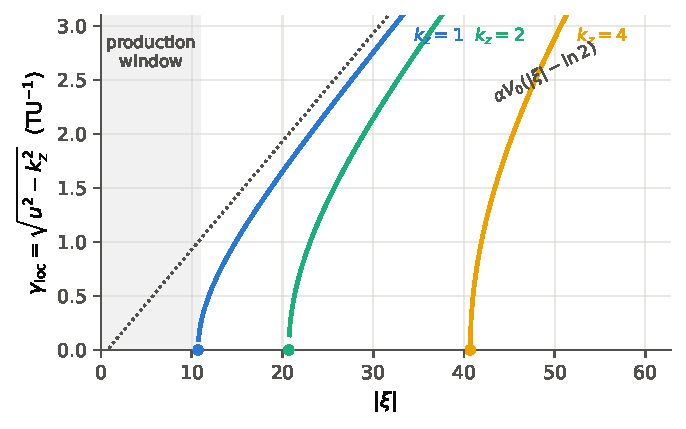
\includegraphics[width=0.62\textwidth]{fig_tachyon.pdf}
\caption{The tachyonic local envelope \eqref{eq:gloc} at $\alpha=2$,
$\Vo=0.05$ for three $\kz$. Dots on the axis mark the critical radii
\eqref{eq:xicrit}; the dotted line is the linear asymptote
$\alpha\Vo(|\xi|-\ln2)$. Higher $\kz$ pushes the instability outward
--- which is why a production window (shaded, $\xi_w=11$) can exclude
the branch entirely for the measured modes, and why the exclusion fails
at large $\alpha$ (Corollary~\ref{cor:highalpha}).}
\label{fig:tachyon}
\end{figure}

\begin{step}[Finite $k_x$ only subtracts]
Keep $k_x\neq0$ but drop the charge coupling (outer region, $v$ at its
plateau; the charge terms decouple from the growing branch --- verified
numerically at all outer eigenmode peaks). Then
\eqref{eq:sixfield} retains $e_z$: from
$\gamma e_z=\ii k_xb$, $\gamma b=-\ii\OmF e_x+\ii k_xe_z$,
$\gamma e_x=-\ii\OmA b$:
\begin{equation}
\gamma^2b=-\ii\OmF(\gamma e_x)+\ii k_x(\gamma e_z)
=-\OmA\OmF\,b-k_x^2\,b
\quad\Longrightarrow\quad
\gamma^2=u^2-\kz^2-k_x^2 .
\label{eq:tachyonkx}
\end{equation}
$\gamma_{\mathrm{loc}}(\xi)$ of \eqref{eq:gloc} is therefore the
\emph{pointwise envelope} over all $x$-structures; global modes must
oscillate ($k_x^2>0$ costs growth) and sit below it.
\end{step}

\begin{intuition}
An effective wavenumber crossing zero. A wave with
$k_{z,\mathrm{eff}}^2=\kz^2-u^2<0$ has an imaginary wavenumber --- as in
an overdense plasma, but with the roles inverted: it is the
\emph{restoring} term of the wave operator that changes sign, so instead
of evanescing in space the mode grows in time, rolling down an inverted
potential. And it is the same shift $u$ that, inside
$\xi_{\mathrm{crit}}$, deepens the confining well of the shear branch
(through $\D$ in \S\ref{sec:reduction}): one term, two fates, split at
$\xi_{\mathrm{crit}}$. Window design is nothing more than choosing which
side of $\xi_{\mathrm{crit}}$ the simulation keeps.
\end{intuition}

\begin{remark}[Energy source and the freeze artifact]
By \eqref{eq:batterysign}, this branch is powered entirely by the frozen
$\Az$; the model as posed makes it a true linear instability with a
bottomless supply. Its runaway character (not its existence) is the freeze
artifact; windows (sponge/cut) placed inside $\xi_{\mathrm{crit}}$ are the
legitimate excision of this branch from shear-physics measurements. The
self-consistent test (\S\ref{ssec:backreaction}) shows the unfrozen
back-reaction does not deplete the background either --- it deepens it
locally and stabilizes only weakly and globally.
\end{remark}

\begin{cor}[High-$\alpha$ window collapse]
\label{cor:highalpha}
A window of radius $\xi_w$ excludes the tachyonic branch only if
$\xi_w<\xi_{\mathrm{crit}}=\kz/(\alpha\Vo)+\ln2$. As $\alpha$ grows at
fixed $\kz,\Vo$, $\xi_{\mathrm{crit}}\to\ln2$: eventually \emph{no} window
can both contain the shear-branch well (which needs $\xi_w$ of order
several) and exclude the tachyon. This is the mechanism of the early
tachyonic blow-ups in the $\alpha\ge6$ corner of the EPS-scan~v2 campaign:
at $\alpha=6$, $\Vo=0.05$, $\kz=2$, $\xi_{\mathrm{crit}}=7.4$, already
inside the vetted windows, and the failure maps to $\alpha$, not $\kz$,
exactly as \eqref{eq:xicrit} predicts.
\end{cor}

\begin{remark}[The ``precession cascade'' scale $\gamma_{\mathrm{casc}}
\approx\alpha\Vo$]
Near the layer ($|\xi|=\mathcal O(1)$, $|\Az|\lesssim\Vo$), the same
color-mixing terms rotate the color-2/3 sector at the local rate
$\alpha|\Az|\sim\alpha\Vo$. Seeding campaigns observed the resulting
build-up of $A_z^{2,3}$ at $\gamma_{\mathrm{casc}}\approx\alpha\Vo$
($0.20$--$0.24$ at $\alpha=2$, $\Vo=0.1$), which can mask slower KH growth
--- the motivation for eigenfunction seeding (\S\ref{sec:seeding}). It is
the same mechanism as \eqref{eq:tachyon} evaluated at the layer-scale
$|\Az|$ rather than the outer plateau.
\end{remark}

\subsection{Charge block: the local drive branch}
\label{ssec:chargeblock}

\begin{step}[Solve the two precession equations]
From \eqref{eq:chargeblock},
\begin{equation}
q_A=\frac{\ii\alpha v\,a}{\gamma+\ii v\OmA},\qquad
q_B=\frac{\ii\alpha v\,a}{\gamma-\ii v\OmA}.
\label{eq:qsol}
\end{equation}
\end{step}

\begin{step}[Beam-difference response]
\begin{equation}
q_A-q_B=\ii\alpha v a
\left[\frac{1}{\gamma+\ii v\OmA}-\frac{1}{\gamma-\ii v\OmA}\right]
=\ii\alpha v a\;\frac{-2\ii v\OmA}{\gamma^2+v^2\OmA^2}
=\frac{2\alpha v^2\OmA}{\R}\;a,
\qquad
\R\equiv\gamma^2+v^2\OmA^2 .
\label{eq:qdiff}
\end{equation}
\end{step}

\begin{step}[Close through $e_z$ and $a$]
$\gamma e_z=v(q_A-q_B)=\dfrac{2\alpha v^3\OmA}{\R}a\equiv g\,a$ and
$e_z=-\gamma a$ give
\begin{equation}
-\gamma^2a=g\,a
\qquad\Longrightarrow\qquad
\boxed{\;\gamma^2=-g,\qquad
g(\xi;\gamma)\equiv\frac{2\alpha v^3\,\OmA}{\gamma^2+v^2\OmA^2}.\;}
\label{eq:localdrive}
\end{equation}
On the side of the layer where $v^3\OmA<0$, $g<0$ and the block grows:
this is the \emph{local (homogeneous) limit of the shear-branch drive}.
The function $g$ defined here is exactly the drive that appears in the
reduced ODE (\S\ref{sec:reduction}); equation \eqref{eq:localdrive} is its
$k_x\to0$ limit, and its maximization over the background will produce the
growth ceiling in \S\ref{sec:ceiling}.
\end{step}

\begin{intuition}
The charge block is a pair of driven pendulums. The potential $a$ shakes
each beam's color charge (the $\ii\alpha v a$ source); each charge then
precesses in the background at its own Doppler-shifted frequency
$\pm v\OmA$ (opposite for the two beams). Their \emph{difference} is what
radiates, through the current $-v(q_A-q_B)$, and it feeds $a$ back with a
sign set by which beam leads in phase. Growth is a phase-locking
phenomenon between the wave and the beams' color precession --- the
resonance structure this implies is made exact in \S\ref{sec:ceiling}.
\end{intuition}

\subsection{Airy estimate for wall-bounded outer modes}
\label{ssec:airy}

Global tachyonic modes live in the annulus between $\xi_{\mathrm{crit}}$
and the window radius $\xi_w$ (hard cut: Dirichlet wall). Their rates
follow from a one-dimensional bound-state problem in the local potential
$U(x)\equiv\gamma_{\mathrm{loc}}^2(x)$, increasing outward:
\begin{equation}
a''+\bigl(U(x)-\gamma^2\bigr)a=0 ,
\end{equation}
with $a=0$ at the wall $x_w$ and decay toward the layer.

\begin{step}[Linearize at the wall]
Near $x_w$ write $U(x)=U_w-U'\,(x_w-x)$ with $U_w=U(x_w)$,
$U'=\dd U/\dd x>0$. In the inward coordinate $t=x_w-x\ge0$:
\begin{equation}
\frac{\dd^2a}{\dd t^2}-\bigl(\gamma^2-U_w+U'\,t\bigr)a=0 .
\end{equation}
\end{step}

\begin{step}[Airy form]
Substitute $\tau=(U')^{1/3}t+\tau_0$ with
$\tau_0=(\gamma^2-U_w)/(U')^{2/3}$:
\begin{equation}
\frac{\dd^2a}{\dd\tau^2}=\tau\,a ,
\end{equation}
whose solution decaying for $\tau\to+\infty$ (deep inside, where
$U<\gamma^2$) is $\mathrm{Ai}(\tau)$.
\end{step}

\begin{step}[Wall condition]
The Dirichlet wall at $t=0$ requires $\mathrm{Ai}(\tau_0)=0$. The least
negative zero of $\mathrm{Ai}$ is $-a_1=-2.338\ldots$, so the deepest
(fastest) mode has $\tau_0=-a_1$:
\begin{equation}
\boxed{\;
\gamma^2\simeq U_w-2.338\,(U')^{2/3}
\;}
\label{eq:airy}
\end{equation}
\end{step}

\begin{cor}[Why tight windows kill the branch outright]
For a tight window, $U_w=\gamma_{\mathrm{loc}}^2(\xi_w)$ is small (the wall
sits just past $\xi_{\mathrm{crit}}$) while the slope
$U'\simeq2(\alpha\Vo)^2(\xi_w-\ln2)/\eps$ is not; \eqref{eq:airy} then goes
\emph{negative}: the annulus holds no bound state at all, and windowing
does not merely reduce the outer branch --- it removes it
(Fig.~\ref{fig:airy}). Measured global
rates at the widest tested annuli reach $0.78\times$ the envelope with a
discrete ladder below, in line with the quantization cost in
\eqref{eq:airy}.
\end{cor}

\begin{figure}[t]
\centering
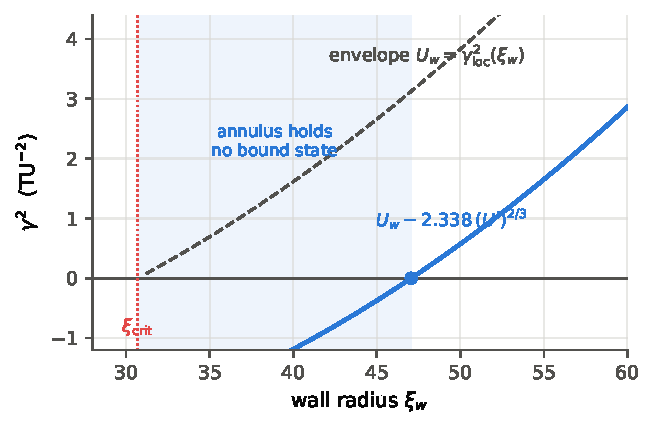
\includegraphics[width=0.60\textwidth]{fig_airy.pdf}
\caption{The Airy wall estimate \eqref{eq:airy} for outer modes bounded
by a hard cut at $\xi_w$ ($\alpha=1$, $\Vo=0.05$, $\kz=1.5$,
$\eps=0.15$). The dashed curve is the pointwise envelope
$U_w=\gamma_{\mathrm{loc}}^2(\xi_w)$; the solid curve subtracts the
quantization cost $2.338\,(U')^{2/3}$ of bending the mode to zero at the
wall. In the shaded range of wall radii the corrected $\gamma^2$ is
negative: the annulus between $\xi_{\mathrm{crit}}$ and the wall is too
narrow to hold any bound state, which is why tight windows remove the
outer branch outright rather than merely weakening it.}
\label{fig:airy}
\end{figure}
% ==============================================================================
\section{Exact scalar reduction of the six-field system}
\label{sec:reduction}

The six-field system \eqref{eq:sixfield} contains only one $x$-derivative
chain ($e_z'\to b\to b'$); everything else is algebraic. It therefore
reduces \emph{exactly} to one second-order ODE for the potential amplitude
$a(x)$. This reduction, verified to machine precision against the ARPACK
eigenvalues of the discrete six-field operator, is the backbone of the
exact-action theory.

\subsection{Continuum elimination}
\label{ssec:elimination}

\begin{step}[Eliminate $e_x$]
From \eqref{eq:lin-ex}: $e_x=-\ii\OmA b/\gamma$.
\end{step}

\begin{step}[Eliminate $e_z$]
From \eqref{eq:lin-a}: $e_z=-\gamma a$.
\end{step}

\begin{step}[Express $b$ through $a'$]
Insert both into Faraday \eqref{eq:lin-b}:
\begin{equation}
\gamma b=-\ii\OmF\Bigl(-\frac{\ii\OmA}{\gamma}b\Bigr)+(-\gamma a)'
=-\frac{\OmA\OmF}{\gamma}\,b-\gamma\,a' .
\end{equation}
Multiply by $\gamma$ and collect $b$:
\begin{equation}
b\,\bigl(\gamma^2+\OmA\OmF\bigr)=-\gamma^2a'
\qquad\Longrightarrow\qquad
b=-\frac{\gamma^2\,a'}{\D},
\qquad
\boxed{\;\D(x)\equiv\gamma^2+\OmA\OmF=\gamma^2+\kz^2-u(x)^2\;}
\label{eq:bfroma}
\end{equation}
$\D$ is the electromagnetic factor: $\D<0$ is exactly the tachyonic region
of \S\ref{ssec:tachyon} (one polarization sees a negative effective
$k^2$); the shear branch lives where $\D>0$.
\end{step}

\begin{step}[Charge response]
Equations \eqref{eq:qsol}--\eqref{eq:qdiff} hold pointwise with
$v=v(\xi)$, $\OmA=\OmA(\xi)$:
\begin{equation}
q_A-q_B=\frac{2\alpha v^2\OmA}{\R}\,a,
\qquad \R(x)=\gamma^2+v^2\OmA^2 .
\end{equation}
\end{step}

\begin{step}[Assemble Amp\`ere-$z$]
Insert $e_z=-\gamma a$, \eqref{eq:bfroma} and the charge response into
\eqref{eq:lin-ez}:
\begin{equation}
-\gamma^2a
=\Bigl(-\frac{\gamma^2a'}{\D}\Bigr)'+\frac{2\alpha v^3\OmA}{\R}\,a
\end{equation}
and rearrange:
\begin{equation}
\boxed{\;
\Bigl(\frac{\gamma^2\,a'}{\D}\Bigr)'=\bigl(\gamma^2+g\bigr)\,a,
\qquad
g(x)=\frac{2\alpha\,v^3\,\OmA}{\gamma^2+v^2\OmA^2}\;}
\label{eq:reduced}
\end{equation}
--- one Sturm--Liouville-type equation, nonlinear in the eigenvalue
$\gamma$ (which appears in $\D$, $g$, and the right side), but scalar.
(``Sturm--Liouville'' is only the mathematicians' name for the flux-form
structure $(p\,a')'=W\,a$ that the stationary Schr\"odinger equation
also has; nothing deeper is implied by the term. The next subsection
unpacks the analogy at length.)
\end{step}

\subsection{How to read the reduced equation: a dictionary for the
non-specialist}
\label{ssec:dictionary}

Equation \eqref{eq:reduced} is the pivot of the entire document: every
result that follows --- the ``drive'', the ``resonance'', the
``Lorentzian'' beam response, the growth ``ceiling''
(\S\ref{sec:ceiling}), the ``well'' and its ``quantization''
(\S\ref{sec:quant}) --- is a statement about this one ODE. That
vocabulary is second nature in plasma physics and quantum mechanics but
is jargon to everyone else, and until now it has not been earned by the
text. This subsection therefore builds each term explicitly from three
pieces of a standard bachelor's curriculum: the finite potential well,
the driven damped oscillator, and spin precession in a magnetic field.
Readers already fluent in the vocabulary can skip to
\S\ref{ssec:anatomy} without loss --- nothing here is used as a
technical ingredient later, only as language.

\paragraph{The reduced equation is a Schr\"odinger eigenvalue problem in
disguise.}
Recall the stationary Schr\"odinger equation for a particle in a
one-dimensional potential, written with everything on one side:
\begin{equation}
\psi''(x)=\frac{2m}{\hbar^2}\bigl[V(x)-E\bigr]\,\psi(x).
\label{eq:schrodinger}
\end{equation}
Its qualitative behavior is controlled entirely by the sign of the
bracket. Where $E>V$ (the \emph{classically allowed} region) $\psi$
oscillates in $x$; where $E<V$ (\emph{forbidden} region) $\psi$ grows or
decays exponentially. A \emph{well} is an allowed region sandwiched
between forbidden ones; a \emph{bound state} is a solution that decays
into the forbidden regions on both sides; and requiring the oscillation
inside the well to join smoothly onto decay outside is possible only at
discrete values of $E$ --- that matching condition is all that
\emph{quantization} means, here and in every later section.

Equation \eqref{eq:reduced} has exactly this structure, with two
differences. First, the second derivative appears in ``flux form'',
$(\gamma^2a'/\D)'$, with a position-dependent coefficient --- the same
form the Schr\"odinger equation takes for a position-dependent mass, or
the steady heat-conduction equation for a position-dependent
conductivity. This changes bookkeeping (the $\D$ factors tracked in
\S\ref{ssec:anatomy}) but not the oscillate-versus-decay dichotomy. The
precise analogue of the bracket $\tfrac{2m}{\hbar^2}[V-E]$ --- the
single function of $x$ whose sign separates oscillation from decay ---
is written down in \S\ref{ssec:anatomy}, eq.~\eqref{eq:Qexact}, as
$-Q(x;\gamma)$. Second, and less trivially, the eigenvalue $\gamma$
does not enter linearly the way $E$ does: it is buried inside $\D$,
inside $g$, and on the right-hand side. In practice such a problem is
solved iteratively (guess $\gamma$, solve the resulting \emph{linear}
well problem, correct $\gamma$, repeat --- this is what the Newton
iteration of \S\ref{ssec:discrete} does), and none of the
well/bound-state/quantization reasoning is affected.

\paragraph{What is being solved for.}
Every perturbation was assumed to evolve as $e^{\gamma t}$
(\S\ref{sec:sixfield}), so a solution with $\gamma>0$ is an
exponentially growing wave --- an instability. The role of the energy
eigenvalue $E$ is played by the growth rate: instead of asking ``which
energies admit a bound state?'' one asks ``which growth rates admit a
trapped, self-consistently growing wave profile?''. The largest such
$\gamma$ is what the simulation measures, because after a few
$e$-foldings the fastest exponential dominates regardless of how the
initial condition distributed amplitude among the modes.

\paragraph{What ``drive'' means.}
Look at the right-hand side of \eqref{eq:reduced}, $(\gamma^2+g)\,a$.
If $g$ were zero, the bracket would be positive everywhere, and
(wherever $\D>0$) the equation would admit only exponential $x$-profiles
--- forbidden region everywhere, no trapped mode, no instability. A well
can open only where $g$ is \emph{negative and exceeds $\gamma^2$ in
magnitude}. So $g$ is the one term that makes growth possible: it
measures how strongly the beams' collective response feeds energy back
into the wave, and it is called the \emph{drive} in exactly the sense of
the driving force of a forced oscillator. Its microscopic origin is the
color current $\delta J_z=-v\,(q_A-q_B)$ of the beams' perturbed
charges, which entered Amp\`ere-$z$ in \eqref{eq:lin-ez}; a growing mode
is a wave that digs its own potential well out of the beam response and
then lives in it.

\paragraph{Where the response denominator $\R$ comes from: a
driven-precession toy problem.}
The building block of $g$ is the beam response \eqref{eq:qsol}, and it
is worth deriving once in stripped-down notation. Let a single complex
variable $q(t)$ obey
\begin{equation}
\frac{\dd q}{\dd t}=-\ii\,\Omega_{\mathrm{prec}}\,q+S\,e^{\gamma t}.
\label{eq:toyprec}
\end{equation}
With $S=0$ the solution is $q\propto e^{-\ii\Omega_{\mathrm{prec}}t}$:
free rotation of the complex phase at frequency
$\Omega_{\mathrm{prec}}$. This is mathematically identical to a magnetic
moment precessing about a static magnetic field (Larmor precession); in
our problem the background potential plays the role of the field and the
beam's color charge plays the role of the moment --- the precession
equations \eqref{eq:lin-qA}--\eqref{eq:lin-qB} are precisely of this
form with $\Omega_{\mathrm{prec}}=\pm v\OmA$, the sign differing between
the beams because they stream in opposite directions. Now switch on the
forcing $S\,e^{\gamma t}$ (the wave $a$ shaking the charge) and look for
the driven response $q=C\,e^{\gamma t}$:
\begin{equation}
\gamma\,C=-\ii\Omega_{\mathrm{prec}}\,C+S
\quad\Longrightarrow\quad
C=\frac{S}{\gamma+\ii\,\Omega_{\mathrm{prec}}},
\qquad
|C|^2=\frac{|S|^2}{\gamma^2+\Omega_{\mathrm{prec}}^2}.
\label{eq:toyresponse}
\end{equation}
This two-line calculation \emph{is} \eqref{eq:qsol}, and the
beam-difference algebra of \eqref{eq:qdiff} then produces the
denominator $\R=\gamma^2+v^2\OmA^2$ that recurs everywhere afterwards.
Note the role played by $\gamma$: it sits where a damping rate would sit
in the classical driven-oscillator formula. Not because anything is
dissipated --- the model is dissipation-free --- but because a signal
growing as $e^{\gamma t}$ is not a pure sinusoid: over one $e$-folding
time $1/\gamma$ it cannot distinguish precession phases within a band of
width $\sim\gamma$, so the response is smeared over that bandwidth
exactly as damping smears a classical resonance.

\paragraph{``Lorentzian'' is the name of a curve, not of a group.}
The bell-shaped function
\begin{equation}
L(\Omega)=\frac{1}{\gamma^2+\Omega^2}
\label{eq:lorentzian}
\end{equation}
--- peak height $1/\gamma^2$ at $\Omega=0$, half-width $\gamma$ --- is
called a \emph{Lorentzian}, after H.~A.~Lorentz's classical model of
spectral-line broadening. It is the universal response curve of a driven
system with finite bandwidth: the resonance curve of the damped driven
oscillator, the shape of atomic and laser spectral lines, the
Breit--Wigner resonance shape of particle physics, the NMR absorption
line. Its odd companion $\Omega\,L(\Omega)=\Omega/(\gamma^2+\Omega^2)$,
with extrema at $\Omega=\pm\gamma$, is the standard \emph{dispersive}
line shape of resonance physics. When \S\ref{sec:ceiling} says ``the
beam response is a Lorentzian in the local precession frequency'', it
means precisely that $1/\R$ is the curve $L$ evaluated at
$\Omega=v\OmA$; the drive $g$, which carries one extra factor of the
precession frequency (the beam \emph{difference} of \eqref{eq:qdiff}
vanishes at $\OmA=0$), is the dispersive companion. The word has nothing
to do with Lorentz transformations, boosts, or the Lorentz group.

\begin{intuition}
The whole instability in one paragraph. The wave $a$ shakes each beam's
color charge (the source $\ii\alpha v\,a$ in \eqref{eq:lin-qA}); each
charge precesses about the color-1 background like a magnetic moment
about a static field, at the Doppler-shifted rate $\pm v\OmA$; because
the beams stream oppositely they precess in opposite senses, so their
responses differ; the difference is a net color current
$\delta J_z=-v(q_A-q_B)$; and that current feeds back into the wave
through Amp\`ere's law. Where the feedback arrives with the right phase
the loop has gain ($g<0$), the wave digs its own well and grows inside
it. Everything that follows quantifies this loop:
\S\ref{ssec:anatomy} reads off which factors control the gain,
\S\ref{sec:ceiling} finds where the gain is largest (a resonance) and
how large it can possibly be (the ceiling $\gamma^3\le\alpha\Vo^2$), and
\S\ref{sec:quant} determines which wave shapes fit inside the well
(quantization).
\end{intuition}

\subsection{Anatomy of the reduced equation}
\label{ssec:anatomy}

With the dictionary of \S\ref{ssec:dictionary} in hand,
eq.~\eqref{eq:reduced} can be read factor by factor.

\begin{intuition}
Why three powers of $v$. The wave must, in order: (i) \emph{shake} the
charges --- only moving beams feel the precession source, one factor of
$v$; (ii) make the two beams respond \emph{differently} --- otherwise
their currents cancel, and the only asymmetry between them is their
opposite Doppler rotation, a second factor of $v$; (iii) \emph{collect}
the response as a current, $\delta J_z=-v(q_A-q_B)$, a third factor of
$v$. The drive therefore dies as $v^3$ toward the layer center: the shear
branch is anchored to the \emph{flow}, not to the field maximum. Its
one-sidedness is helicity selection --- each circular polarization
couples to the side whose flow direction matches its rotation sense,
and the mirror mode belongs to the conjugate polarization
(\S\ref{ssec:helicity}).
\end{intuition}

\begin{itemize}
\item \textbf{$\D$ (EM factor).} Sign changes of $\D$ separate the
propagating/trapped shear-branch region from the tachyonic outer region:
one mechanism --- the covariant shift $u$ --- creates both the confining
well and, past $|\xi|=\xi_{\mathrm{crit}}$, the runaway. (``The well and
the tachyon are two sides of one term.'')
\item \textbf{$g$ (drive).} The \emph{only} drive of the shear branch, and
precisely the local-drive function of \eqref{eq:localdrive}. Its three
powers of $v$ have distinct origins: one from the precession source
($\ii\alpha va$ in \eqref{eq:lin-qA}), one from the beam Doppler asymmetry
(the $v\OmA/\R$ structure of \eqref{eq:qdiff}), one from the current
($\delta J_z=-v(q_A-q_B)$). Counter-streaming enters only through the even
combination $\R=\gamma^2+v^2\OmA^2$.
\item \textbf{One-sidedness.} $g\propto v^3$ is odd in $\xi$ (for
$\OmA>0$): each circular polarization is driven on one side of the layer
only; the mirror image is carried by the conjugate polarization at the
same $|\gamma|$ (\S\ref{ssec:helicity}). This explains the one-sided
eigenfunctions seen in all solver outputs.
\item \textbf{WKB form.} Writing $a\propto\exp(\pm\ii\int\!\sqrt{Q}\,\dd x)$
brings \eqref{eq:reduced} to the standard form with the exact local
wavenumber
\begin{equation}
\boxed{\;Q(x;\gamma)=-\,\frac{\D\,\bigl(\gamma^2+g\bigr)}{\gamma^2}\;}
\label{eq:Qexact}
\end{equation}
(the flux form contributes the $\D$ weight; a well requires $Q>0$, i.e.\
$\D>0$ together with $g<-\gamma^2$).
\end{itemize}
Figure~\ref{fig:anatomy} displays $\D$ and $Q$ at a production point,
computed at the model-B eigenvalue.

\begin{figure}[t]
\centering
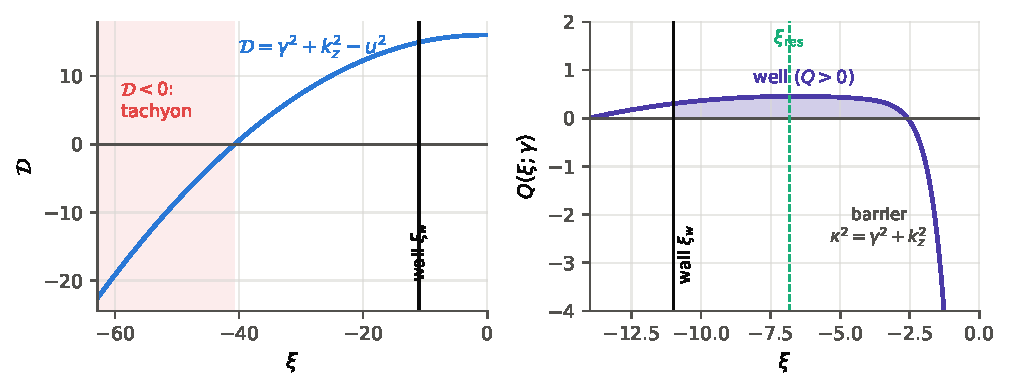
\includegraphics[width=\textwidth]{fig_anatomy.pdf}
\caption{Anatomy of the reduced equation \eqref{eq:reduced} on the driven
side ($\alpha=2$, $\Vo=0.05$, $\eps=0.15$, $\kz=4$, cut $\xi_w=11$,
$\gamma=0.1694$ from model B). \emph{Left}: the EM factor $\D$ over the
whole half-box; $\D<0$ (shaded) beyond $\xi_{\mathrm{crit}}\approx-41$
is the tachyonic region --- far outside the wall, which is the point of
the window. \emph{Right}: the exact local wavenumber $Q(\xi;\gamma)$ of
\eqref{eq:Qexact} near the layer: the shallow well ($Q>0$, shaded)
between the wall and the tanh$^3$ knee, the resonance surface
$\xi_{\mathrm{res}}$ of \eqref{eq:xires} inside it, and the strong
evanescent barrier ($Q\to-(\gamma^2+\kz^2)$, off scale) toward the
layer. The shallowness of the well --- it holds less than a quarter
wavelength --- is the quantization marginality of \S\ref{sec:quant}.}
\label{fig:anatomy}
\end{figure}

\subsection{Exactness at the discrete level; the two wall faces}
\label{ssec:discrete}

The eigensolver uses a forward difference for $\partial_xe_z$ (Faraday
row) and a backward difference for $\partial_xb$ (Amp\`ere-$z$ row),
matching the simulation's Yee stagger. Repeat the elimination on the
lattice ($x_i=i\,\dd x$):

\begin{step}
The discrete Faraday/Amp\`ere-$x$ pair gives, per node $i$,
\begin{equation}
b_i\,\frac{\D_i}{\gamma}=\frac{e_{z,i+1}-e_{z,i}}{\dd x}
\;\Longrightarrow\;
b_i=-\frac{\gamma^2}{\D_i}\,\frac{a_{i+1}-a_i}{\dd x},
\end{equation}
i.e.\ $b_i$ lives on the \emph{face} between nodes $i$ and $i{+}1$, with
$\D$ evaluated at the left node of the face.
\end{step}

\begin{step}
The discrete Amp\`ere-$z$ row then reads
\begin{equation}
-\gamma^2a_i=\frac{b_i-b_{i-1}}{\dd x}+g_ia_i
=-\frac{\gamma^2}{\dd x^2}
\left[\frac{a_{i+1}-a_i}{\D_i}-\frac{a_i-a_{i-1}}{\D_{i-1}}\right]+g_ia_i ,
\label{eq:discretereduced}
\end{equation}
the exact flux-form finite difference of \eqref{eq:reduced}. No
approximation was made: the $6N\times6N$ eigenproblem and the $N\times N$
nonlinear problem \eqref{eq:discretereduced} have identical spectra on the
shared modes. Verified: Newton iteration on \eqref{eq:discretereduced}
reproduces the six-field ARPACK eigenvalues to relative difference $0.0$
(below $10^{-10}$) at seven points spanning $\alpha=1$--$3$,
$\Vo=0.03$--$0.1$, $\kz=1$--$7$.
\end{step}

\begin{step}[Wall faces]
A hard cut (\texttt{xi\_cut}) zeroes all fields outside radius $\xi_w$. In
the reduction the two sides of the wall behave differently:
\begin{itemize}
\item where the \emph{right} neighbor is outside, $e_{z,i+1}$ is a
Dirichlet ghost ($e_z=0$, hence $a=0$): the face flux uses a zero value
--- a Dirichlet face;
\item where the \emph{left} neighbor is outside, $b_{i-1}$ is dropped:
the face flux itself vanishes --- a zero-flux (Neumann, $b=0\equiv a'=0$)
face.
\end{itemize}
The mode side of the wall is therefore Neumann for $a$, the far side
Dirichlet; the two faces are \emph{not} equivalent, and the Neumann
condition on the mode side is what enters the quantization phase in
\S\ref{sec:quant}.
\end{step}

% ==============================================================================
\section{The drive: precession resonance, the growth ceiling, and natural
units}
\label{sec:ceiling}

The plan of this section, in plain language.
\S\ref{sec:reduction} ended with a wave trapped in a well whose depth is
set by the drive $g$, together with the criterion (below
\eqref{eq:Qexact}) that a well exists only where $-g>\gamma^2$. Two
elementary questions therefore control everything. \emph{Where}, as a
function of position, is the drive strongest? Answered in
\S\ref{ssec:resonance} by maximizing a function of one variable: on a
\emph{resonance surface}, where the beam-frame precession frequency
matches the growth rate. \emph{How strong} can the drive possibly be?
The maximum turns out to be $\alpha\Vo^2/\gamma$, and inserting it into
the well-existence criterion bounds the growth rate of \emph{every}
mode by $\gamma^3\le\alpha\Vo^2$ --- the ceiling, which the measured
dispersion peaks saturate to within a few percent. No new physics
enters this section: it is first-year calculus applied to the drive $g$
of \eqref{eq:reduced}.

\subsection{The saturated drive $G(w)$}
\label{ssec:G}

\begin{step}[Specialize $g$ to the saturation plateaus]
The drive $g(x)=2\alpha v^3\OmA/(\gamma^2+v^2\OmA^2)$ of
\eqref{eq:reduced} contains two background profiles, $v(\xi)$ and
$\OmA(\xi)=\kz-u(\xi)$. For $|\xi|\gtrsim2$ both simplify: the shear is
saturated, $v=\pm\Vo$ (so $v^2=\Vo^2$ exactly), and $u$ grows linearly,
$u=\alpha\Vo(|\xi|-\ln2)$ by \eqref{eq:usat}. All position dependence of
$g$ then enters through the single combination
\begin{equation}
w\equiv\OmA(\xi)=\kz-u(\xi),
\label{eq:wdef}
\end{equation}
the \emph{local covariant wavenumber}: the wavenumber the wave
effectively carries at position $\xi$ after the background's
minimal-coupling shift (\S\ref{sec:sixfield}). At the layer $u\approx0$,
so $w\approx\kz$; moving outward, $w$ \emph{decreases linearly} with
$|\xi|$ at slope $\alpha\Vo$, crossing zero at
$|\xi|=\xi_{\mathrm{crit}}$ \eqref{eq:xicrit}. On each plateau, position
and $w$ are thus interchangeable coordinates, and any statement about
the best $w$ translates directly into the position $\xi$ where that $w$
is attained (\S\ref{ssec:xires}).
\end{step}

\begin{step}[Sign bookkeeping: which side of the layer drives]
A well needs $g<0$ (\S\ref{ssec:dictionary}), and the sign of $g$ is the
sign of $v^3\OmA$. Between the layer and $\xi_{\mathrm{crit}}$, where
$w=\OmA>0$, this requires $v<0$: for the $2+\ii3$ polarization the
driven side is $\xi<0$. (The other side is not lost --- by the
helicity--parity symmetry of \S\ref{ssec:helicity} it carries the mirror
mode of the conjugate polarization at exactly the same growth rate, so
studying one side loses no generality.) On the driven side $v=-\Vo$,
hence $v^3=-\Vo^3$, and the \emph{magnitude} of the drive is
\begin{equation}
-g=G(w)\equiv\frac{2\alpha \Vo^3\,w}{\gamma^2+\Vo^2w^2},
\qquad w>0 .
\label{eq:Gdef}
\end{equation}
\end{step}

\begin{step}[Shape of $G$: weak when slow, weak when fast]
$G$ is the dispersive Lorentzian of \S\ref{ssec:dictionary} in the
precession frequency $\Vo w$, and its two limits have transparent
physical readings:
\begin{itemize}
\item $\Vo w\ll\gamma$ (slow precession):
$G\simeq(2\alpha\Vo^3/\gamma^2)\,w\to0$. At $w=0$ the two beams'
precession frequencies $\pm\Vo w$ both vanish, the beams respond
identically, and their currents cancel ($q_A-q_B\to0$ in
\eqref{eq:qdiff}): no beam asymmetry, nothing to feed the wave.
\item $\Vo w\gg\gamma$ (fast precession): $G\simeq2\alpha\Vo/w\to0$. The
charges now turn through many radians during one $e$-folding time
$1/\gamma$ of the wave; their response averages out over the fast
rotation and little net work is done.
\end{itemize}
Between the two limits $G$ must peak --- the resonance, located next.
\end{step}

\subsection{Resonance and the exact ceiling}
\label{ssec:resonance}

\begin{step}[Maximize $G$ over $w$]
\begin{equation}
\frac{\dd G}{\dd w}
=2\alpha\Vo^3\,\frac{(\gamma^2+\Vo^2w^2)-w\,(2\Vo^2w)}{(\gamma^2+\Vo^2w^2)^2}
=2\alpha\Vo^3\,\frac{\gamma^2-\Vo^2w^2}{(\gamma^2+\Vo^2w^2)^2}=0
\;\Longrightarrow\;
w^*=\frac{\gamma}{\Vo}.
\label{eq:wstar}
\end{equation}
The condition $\Vo\,w^*=\gamma$ says: the mode grows fastest where the
\emph{beam-frame precession frequency} $v\,\OmA=\Vo w$ matches the growth
rate --- a precession resonance surface in the flow. The peak value is
\begin{equation}
G_{\max}=G(w^*)=\frac{2\alpha\Vo^3\,(\gamma/\Vo)}{2\gamma^2}
=\frac{\alpha\Vo^2}{\gamma}.
\label{eq:Gmax}
\end{equation}
\end{step}

\begin{step}[Ceiling, derivation 1 (well existence)]
By \eqref{eq:Qexact}, a confining well ($Q>0$ with $\D>0$) requires
$g<-\gamma^2$, i.e.\ $G>\gamma^2$ somewhere. Since $G\le G_{\max}$,
\begin{equation}
\gamma^2\le\frac{\alpha\Vo^2}{\gamma}
\qquad\Longleftrightarrow\qquad
\boxed{\;\gamma^3\le\alpha\Vo^2\;}
\label{eq:ceiling}
\end{equation}
independent of $\kz$, $\eps$, and window geometry
(Fig.~\ref{fig:drive}, left).
\end{step}

\begin{intuition}
A self-limiting resonance. The beam response is a Lorentzian
(the resonance line shape of \S\ref{ssec:dictionary}) in the
local precession frequency whose width is set by the growth rate itself
($\R=\gamma^2+v^2\OmA^2$): the faster the mode grows, the broader the
band of precession frequencies it averages over --- exactly as a larger
damping broadens and flattens a classical resonance curve --- and the
weaker the peak drive $G_{\max}=\alpha\Vo^2/\gamma$ it can extract. The ceiling
$\gamma^3=\alpha\Vo^2$ is the fixed point of this self-limitation ---
the mode grows exactly as fast as the drive it leaves itself.
Equivalently, by \eqref{eq:wstar}: the wave can at best grow as fast as
the beams' color charges precess \emph{in the beam frame}; faster growth
would outrun its own energy supply.
\end{intuition}

\begin{step}[Ceiling, derivation 2 (local drive branch)]
Alternatively, the homogeneous charge-block branch \eqref{eq:localdrive}
gives $\gamma^2=G(w)$ pointwise; maximizing the implicit solution over $w$
means solving $\gamma^2=G(w^*)=\alpha\Vo^2/\gamma$, i.e.\
$\gamma=(\alpha\Vo^2)^{1/3}$ exactly. The ceiling is thus the maximum
local growth rate of the drive branch, attained on the resonance surface;
any global (quantized, windowed) mode sits below it. Measured
dominant-branch peaks reach $95$--$99\%$ of $(\alpha\Vo^2)^{1/3}$ in every
validated series.
\end{step}

\subsection{Natural units and the universal well}
\label{ssec:natural}

Define, as in \eqref{eq:scales}, $\Ceil=(\alpha\Vo^2)^{1/3}$,
$\Kwn=(\alpha/\Vo)^{1/3}$, and hatted variables
\begin{equation}
\gamma=\Ceil\,\hat\gamma,\qquad
\kz=\Kwn\,\hat k,\qquad
w=\Kwn\,\hat w,\qquad
u=\Kwn\,\hat u .
\end{equation}

\begin{step}[Scale out the drive]
Using $\Vo^2\Kwn^2=\Vo^2(\alpha/\Vo)^{2/3}=(\alpha\Vo^2)^{2/3}=\Ceil^2$
and $\alpha\Vo^3\Kwn=\alpha^{4/3}\Vo^{8/3}=\Ceil^4$:
\begin{equation}
G(w)=\frac{2\alpha\Vo^3\Kwn\hat w}{\Ceil^2\hat\gamma^2+\Vo^2\Kwn^2\hat w^2}
=\Ceil^2\,\frac{2\hat w}{\hat\gamma^2+\hat w^2}
\;\equiv\;\Ceil^2\,\hat G(\hat w).
\label{eq:Ghat}
\end{equation}
The drive is universal in hatted variables: no $\alpha$, $\Vo$, or $\eps$
remains in $\hat G$.
\end{step}

\begin{step}[Universal well condition and edges]
$G>\gamma^2$ becomes $\hat G>\hat\gamma^2$:
\begin{equation}
\boxed{\;\hat\gamma^2\bigl(\hat\gamma^2+\hat w^2\bigr)<2\hat w\;}
\label{eq:wellhat}
\end{equation}
The edges solve $\hat\gamma^2\hat w^2-2\hat w+\hat\gamma^4=0$:
\begin{equation}
\hat w_\pm=\frac{1\pm\sqrt{1-\hat\gamma^6}}{\hat\gamma^2},
\label{eq:welledges}
\end{equation}
real only for $\hat\gamma\le1$ --- a third, independent derivation of the
ceiling \eqref{eq:ceiling}. As $\hat\gamma\to1$ the well closes onto the
resonance point $\hat w=1$ (i.e.\ $w=\Kwn$, $\gamma/\Vo=\Kwn$); see
Fig.~\ref{fig:drive}, right.
\end{step}

\begin{figure}[t]
\centering
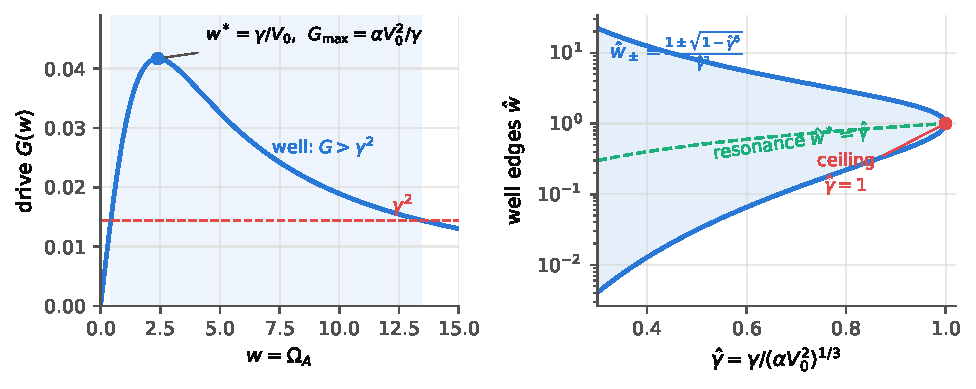
\includegraphics[width=\textwidth]{fig_drive.pdf}
\caption{The precession-resonance drive. \emph{Left}: $G(w)$ of
\eqref{eq:Gdef} at $\alpha=2$, $\Vo=0.05$, $\gamma=0.12$: maximal on the
resonance surface $w^*=\gamma/\Vo$ with $G_{\max}=\alpha\Vo^2/\gamma$
(eq.~\eqref{eq:Gmax}); a confining well exists wherever $G>\gamma^2$
(dashed), the shaded band $w\in(w_-,w_+)$. \emph{Right}: the same in
natural units, eq.~\eqref{eq:welledges}: the well edges $\hat w_\pm$
close onto the resonance point as $\hat\gamma\to1$ --- the graphical
statement of the ceiling $\gamma^3\le\alpha\Vo^2$.}
\label{fig:drive}
\end{figure}

\begin{step}[Provable non-collapse in $\alpha\Vo$]
Rates scale as $(\alpha\Vo^2)^{1/3}$ and wavenumbers as
$(\alpha/\Vo)^{1/3}$: no combination of the two is a function of the
product $\alpha\Vo$ alone. This proved that the survey-era attempt to
collapse the data on $\alpha\Vo$ had to fail, and supplied the variables
for the successful collapse test (T2.5: $\gamma_{\mathrm{peak}}/\Ceil
=0.977\pm0.011$ across $\alpha=1$--$3$, $\Vo=0.03$--$0.1$ at fixed window
group and $\eps=0.15$).
\end{step}

\subsection{The resonance surface in space}
\label{ssec:xires}

Setting $w(\xi)=\kz-u(\xi)=w^*=\gamma/\Vo$ and inverting \eqref{eq:usat}:
\begin{equation}
\boxed{\;
\xi_{\mathrm{res}}\simeq\frac{\kz-\gamma/\Vo}{\alpha\Vo}+\ln2\;}
\label{eq:xires}
\end{equation}
--- the resonance surface moves \emph{outward linearly with $\kz$}. The
eigenmode peak tracks it (measured: peak $\xi$ from $-1$ to $-16$ across
$\kz=0.5$--$10$ at the C25 parameters, $-36$ at cut $40$), which is the
geometric fact behind the confinement-set dispersion peak of
\S\ref{sec:peak}.

% ==============================================================================
\section{Quantization of the shear branch: models A and B}
\label{sec:quant}

First, orientation: which well, and why ``quantize'' it. The well is
the object constructed in \S\ref{sec:reduction} --- the region where
the exact local wavenumber $Q(x;\gamma)$ of \eqref{eq:Qexact} is
positive, so that the wave profile $a(x)$ oscillates in $x$. It is
bounded on the outside by the window wall and on the inside by the
drive shutting off where the shear dies; Fig.~\ref{fig:anatomy} (right
panel) shows one at a production point. In the dictionary of
\S\ref{ssec:dictionary}: allowed region = well; a profile that
oscillates inside it and decays outside it = bound state = the trapped
growing mode we are after. This family of trapped modes is the
\emph{shear branch} (in contrast to the tachyonic \emph{outer} branch
of \S\ref{ssec:tachyon}, which lives beyond $\xi_{\mathrm{crit}}$ and is
excluded by the window). Section~\ref{sec:ceiling} bounded how fast such
a mode \emph{could} grow; it did not determine which $\gamma$ is
actually realized at a given $(\alpha,\Vo,\kz,\text{window})$. That is
fixed by the matching requirement of the dictionary: the oscillation
inside the well must join smoothly onto the decay outside, which is
possible only at special values of $\gamma$. Finding those values is
all that ``quantization'' means here --- the exact analogue of finding
the energy levels of a finite square well in a first quantum-mechanics
course.

Three standard terms, spelled out before use:
\begin{itemize}
\item \textbf{Action.} The total phase the wave accumulates in crossing
the well, $S=\int_{\mathrm{well}}\sqrt{Q}\,\dd x$. It measures how much
wave fits inside: a full wavelength contributes $2\pi$, so $S=\pi/2$
means the well holds a quarter wavelength, $S=\pi$ half a wavelength,
and so on.
\item \textbf{Bohr--Sommerfeld rule.} The textbook WKB result that a
deep well with two smooth (``soft'') edges holds its $n$-th bound state
when $S=(n+\tfrac12)\pi$; the $\tfrac12$ is the sum of two $\pi/4$
phase corrections, one contributed by each soft edge. It presupposes a
well roomy enough to hold at least that much phase.
\item \textbf{Connection conditions.} The bookkeeping at each edge of
the well: the solution's value and slope must be continuous there, and
the \emph{type} of edge --- hard wall, sharp step, or soft turning
point (a point where $Q$ crosses zero with finite slope) --- dictates
the phase with which the interior oscillation must arrive at it.
\end{itemize}

With the vocabulary in place, the one-sentence summary of the section:
\emph{the well is shallow.} At production parameters the measured
action is only $S=0.31\pi$--$0.46\pi$ --- \emph{less than a quarter
wavelength} --- so the Bohr--Sommerfeld rule cannot even be applied
(there is no room for $(n+\tfrac12)\pi$), and the connection conditions
at the two edges do all the work instead. The two models developed
below are two levels of care in applying them: model A
(\S\ref{ssec:modelA}) idealizes the well as a rectangle and closes
everything in one analytic formula; model B (\S\ref{ssec:modelB}) keeps
the exact well shape and solves the matching condition numerically.
Throughout, $n$ labels the rungs of the resulting ladder of solutions:
$n=0$ is the fastest-growing (\emph{dominant}) mode, whose profile has
no zero-crossings inside the well (``nodeless''), and each higher $n$
--- an \emph{overtone} --- fits one extra half-wave into the well and
grows more slowly (\S\ref{ssec:ladder}).

\subsection{Geometry of the well}
\label{ssec:wellgeom}

Fix the driven side of the layer ($\xi<0$ for the $2+\ii3$
polarization, by the sign bookkeeping of \S\ref{ssec:G}). Moving inward
from the wall, the well has the following parts:
\begin{itemize}
\item \textbf{Outer edge}: the window radius $\xi_w$. A hard cut acts
on the mode side as a \emph{zero-flux (Neumann) face}
(\S\ref{ssec:discrete}): the slope of the profile vanishes there,
$a'=0$, so the mode meets the wall with an antinode --- a maximum of
$|a|$, like the open end of an organ pipe. If instead the window is
loose --- so wide that the drive gives out before the wall is reached
--- the outer edge is a \emph{free turning point}: the position where
$Q$ falls through zero because $G$ has dropped back to $\gamma^2$ (the
$w=\hat w_-$ edge of \eqref{eq:welledges}).
\item \textbf{Inner edge}: the ``knee'' $\xi_0$ where the $v^3$ factor
of the drive (the three powers of $v$ dissected in
\S\ref{ssec:anatomy}) switches off over $\lesssim1$ $\xi$-unit as the
shear $v=\Vo\tanh\xi$ dies toward the layer center. Since
$g=-G\,|\tanh\xi|^3$ near the layer-side edge of the saturated region, the
well ends where
\begin{equation}
G\,|\tanh\xi_0|^3=\gamma^2
\qquad\Longrightarrow\qquad
\tanh^3\xi_0=\frac{\gamma^2}{G},
\label{eq:knee}
\end{equation}
giving $\xi_0\approx1.4$--$2$ at production parameters (the code's model~A
uses the fixed representative $\xi_0=1.5$).
\item \textbf{Interior}: the allowed region, $Q>0$ from
\eqref{eq:Qexact}. In the window-limited regime relevant near the
dispersion peak the well sits close to the layer, where the covariant
shift is still small ($u\ll\kz$); then $\D\approx\gamma^2+\kz^2$ and
$G\approx G(\kz)$ vary by $<5\%$ across the well. The coefficients of
the ODE are effectively constant --- the situation of the textbook
finite \emph{square} well, hence the name \emph{square-well regime}
(numerically confirmed at the production points).
\item \textbf{Beyond the inner edge} ($|\xi|<\xi_0$): the drive is
gone, $g\to0$, so $Q\to-\D\approx-(\gamma^2+\kz^2)<0$ --- a forbidden
region, where the profile cannot oscillate but only die off
exponentially (\emph{evanescent}), $a\propto e^{-\kappa s}$ with $s$
the distance into the region and decay constant
\begin{equation}
\kappa=\sqrt{\gamma^2+\kz^2}\;\approx\kz .
\label{eq:kappa}
\end{equation}
\end{itemize}

\subsection{The sharp-edge connection formula}
\label{ssec:connection}

\begin{step}[Interior solution]
Let $k_x=\sqrt{Q}$ (constant in the square-well regime) and measure
distance $s$ inward from the outer wall. Inside the well the general
solution is a combination of $\cos(k_xs)$ and $\sin(k_xs)$; of the two,
only the cosine has zero slope at $s=0$, so the Neumann face ($a'=0$ at
$s=0$, \S\ref{ssec:wellgeom}) selects
\begin{equation}
a(s)=\cos(k_xs).
\end{equation}
\end{step}

\begin{step}[Log-derivative at the inner edge]
Matching value and slope across an edge, when each side carries an
arbitrary overall normalization, is done most economically by matching
the single ratio $a'/a$ (the \emph{logarithmic derivative}), from which
the normalizations cancel. At the inner edge $s=\Delta$ (well width),
with total action $S=k_x\Delta$:
\begin{equation}
\frac{a'}{a}\bigg|_{s=\Delta^-}=-k_x\tan S .
\end{equation}
\end{step}

\begin{step}[Evanescent side]
For $s>\Delta$ the solution decaying toward the layer is
$a\propto e^{-\kappa(s-\Delta)}$ \eqref{eq:kappa}, with $a'/a=-\kappa$.
Both $a$ and $a'$ are continuous at the edge --- a second-order ODE
with finite coefficients cannot support a jump in either --- and
because the drive switches off over a distance short compared with the
interior wavelength $2\pi/k_x$, the coefficient change may be idealized
as a discontinuity (the ``sharp step''), contributing no phase of its
own (unlike the soft turning points met in \S\ref{ssec:modelB}).
Equating the two log-derivatives:
\begin{equation}
-k_x\tan S=-\kappa
\qquad\Longrightarrow\qquad
\boxed{\;\tan S=\frac{\kappa}{k_{\mathrm{edge}}}\;}
\qquad (k_{\mathrm{edge}}=k_x\text{ at the inner edge}),
\label{eq:tanS}
\end{equation}
with $S\in(0,\pi/2)$ for the nodeless $n=0$ mode and $S\in(n\pi,\,
n\pi+\pi/2)$ for the $n$-th overtone. Because $\tan S>0$ requires
$S<\pi/2$ (mod $\pi$), the branch is \emph{quantization-marginal}: it
holds less than a quarter wave, and $\gamma$ adjusts to sit close below
the ceiling so that the well is exactly this shallow. Both the matching
geometry and the graphical solution of model A's closure are shown in
Fig.~\ref{fig:quant}.
\end{step}

\begin{intuition}
A quarter-wave well. The condition is not ``fit $n+\tfrac12$ waves in
the well'' but ``match one shallow cosine arc to its evanescent tail'':
a surface-mode-like state (a wave clinging to an interface rather than
filling a cavity). This marginality explains two robust
observations at once. First, why measured rates hug the ceiling:
lowering $\gamma$ deepens the well quickly (both $G$ and $Q$ rise), so
only a small drop below the ceiling buys all the action the connection
condition demands. Second, why rates are insensitive to window details
(few percent) while the \emph{peak position} is set entirely by them:
$\gamma$ is pinned near the ceiling wherever a well exists at all, and
the geometry only decides for which $\kz$ that is possible
(\S\ref{sec:peak}).
\end{intuition}

\subsection{Model A: closed-form dispersion relation}
\label{ssec:modelA}

Model A adopts the square-well regime literally and closes everything
analytically.

\begin{step}[Assumptions]
(i) $u\ll\kz$ over the well, so $w\approx\kz$ and the drive is the
\emph{Doppler-detuned} value
\begin{equation}
G=G(\kz)=\frac{2\alpha\Vo^3\kz}{\gamma^2+\Vo^2\kz^2}
\label{eq:GofK}
\end{equation}
--- ``detuned'' in the resonance sense of \S\ref{ssec:resonance}: the
well sits where the beams precess at $\Vo\kz$, which is generally
\emph{not} the resonant value $\Vo w^*=\gamma$, so the mode runs on the
off-peak value of the Lorentzian drive rather than on $G_{\max}$;
(ii) $\D\approx\gamma^2+\kz^2$ constant;
(iii) well width $\Delta x=\eps\,(\xi_w-\xi_0)$ with $\xi_0=1.5$.
\end{step}

\begin{step}[Interior wavenumber]
From \eqref{eq:Qexact} with these approximations,
\begin{equation}
k_x=\sqrt{Q}
=\sqrt{\frac{(\gamma^2+\kz^2)(G-\gamma^2)}{\gamma^2}}
=\sqrt{\gamma^2+\kz^2}\;\frac{\sqrt{G-\gamma^2}}{\gamma}
\;\approx\;\kz\,X,
\qquad
\boxed{\;X\equiv\frac{\sqrt{G-\gamma^2}}{\gamma}\;}
\label{eq:Xdef}
\end{equation}
(using $\kz\gg\gamma$ in the prefactor, consistent with (i)).
\end{step}

\begin{step}[Quantization closes on $X$ alone]
Insert $k_x=\kz X$ and $\kappa\approx\kz$ into \eqref{eq:tanS}:
\begin{equation}
S=k_x\,\Delta x=\underbrace{\eps\,(\xi_w-\xi_0)\,\kz}_{\textstyle\equiv L}\;X,
\qquad
\tan S=\frac{\kz}{\kz X}=\frac1X
\quad\Longrightarrow\quad
\boxed{\;L\,X=\arctan\frac1X\;}
\label{eq:LX}
\end{equation}
--- a single transcendental equation for $X$ that contains \emph{no}
$\gamma$: the geometry factor $L$ (window, shear width, wavenumber) fixes
$X$ by itself. $X$ decreases monotonically as $L$ grows (looser window
$\Rightarrow$ smaller interior wavenumber needed).
\end{step}

\begin{step}[Recover $\gamma$]
By the definition of $X$, $G=\gamma^2(1+X^2)$; equate to \eqref{eq:GofK}:
\begin{equation}
\gamma^2\,(1+X^2)\,\bigl(\gamma^2+\Vo^2\kz^2\bigr)=2\alpha\Vo^3\kz .
\end{equation}
This is a quadratic in $\gamma^2$:
\begin{equation}
\gamma^4+\Vo^2\kz^2\,\gamma^2-\frac{2\alpha\Vo^3\kz}{1+X^2}=0 ,
\end{equation}
whose positive root is
\begin{equation}
\boxed{\;
\gamma^2=\tfrac12\left[-\Vo^2\kz^2
+\sqrt{\Vo^4\kz^4+\dfrac{8\alpha\Vo^3\kz}{1+X^2}}\right]
\;}
\label{eq:modelA}
\end{equation}
--- model A. Validated within $\sim3\%$ of the $\sigma$-chased dominant
eigenvalues near and above the dispersion peak, and it identifies the peak
within $\pm0.5$ in $\kz$.
\end{step}

\begin{figure}[t]
\centering
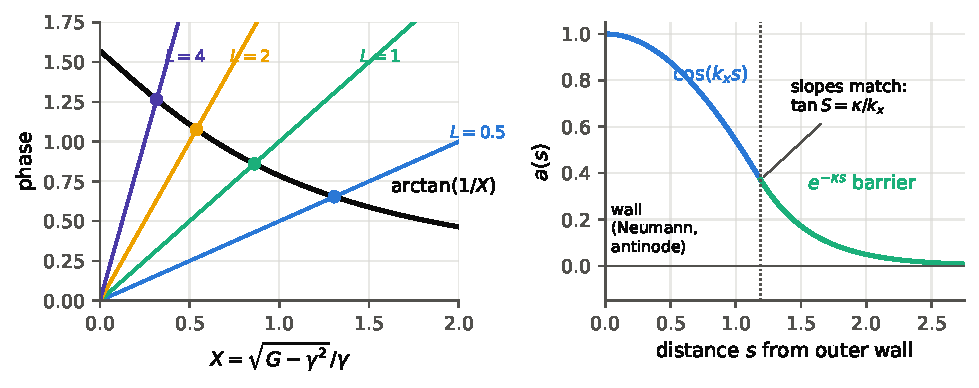
\includegraphics[width=\textwidth]{fig_quant.pdf}
\caption{Quantization mechanics. \emph{Left}: graphical solution of
model A's closure $LX=\arctan(1/X)$, eq.~\eqref{eq:LX} --- the geometry
factor $L=\eps(\xi_w-\xi_0)\kz$ alone fixes the interior-wavenumber
ratio $X$, with no reference to $\gamma$. \emph{Right}: the sharp-edge
matching behind \eqref{eq:tanS} (drawn for $k_x=1$, $\kappa=2.5$): a
cosine arc with its antinode at the Neumann wall meets the evanescent
barrier tail with continuous value and slope, which happens exactly when
$\tan S=\kappa/k_x$; the arc is always shorter than a quarter wave.}
\label{fig:quant}
\end{figure}

\subsection{Model B: exact-action quantization}
\label{ssec:modelB}

Model B keeps the exact $Q(x;\gamma)$ of \eqref{eq:Qexact} --- no
square-well or $w\approx\kz$ approximation --- and root-finds the
quantization phase. For trial $\gamma$:
\begin{enumerate}
\item compute $Q$ on a fine grid of the driven side; find the largest
contiguous region $Q>0$ (the well) inside the window radius $\xi_w$;
\item exact action $S(\gamma)=\int_{\mathrm{well}}\sqrt{Q}\,\dd x$;
\item edge wavenumber $k_{\mathrm{edge}}=\sqrt{Q}$ evaluated just inside
the \emph{inner} edge; $\kappa=\sqrt{\gamma^2+\kz^2}$;
\item connection phase $\Phi$:
\begin{equation}
\Phi=
\begin{cases}
\arctan\bigl(\kappa/k_{\mathrm{edge}}\bigr) &
\text{well attached to the tanh$^3$ knee (sharp inner step)},\\[2pt]
\pi/4 & \text{well detached (soft inner turning point)},
\end{cases}
\label{eq:phases}
\end{equation}
with an additional $+\pi/4$ if the outer edge is a free turning point
rather than the wall, plus $n\pi$ for overtones. Where the $\pi/4$
comes from: at a \emph{soft} edge --- $Q$ crossing zero with finite
slope rather than jumping --- the wave leaks a finite distance into the
forbidden region before dying away, and the standard matched-asymptotics
result (obtained with the same Airy functions used at the wall in
\S\ref{ssec:airy}; any quantum-mechanics text derives it under ``WKB
connection formulas'') is that the interior oscillation must arrive at
such an edge carrying an extra $\pi/4$ of phase. This is precisely the
origin of the $\tfrac12$ in the Bohr--Sommerfeld rule quoted at the top
of this section: a deep well with two soft edges collects
$2\times\pi/4$. Our well replaces one or both soft edges by sharp ones
--- the Neumann wall contributes phase $0$ (cosine antinode at the
wall, exactly as in \eqref{eq:tanS}), and the sharp inner step
contributes the $\arctan$ of \eqref{eq:tanS} instead of $\pi/4$ ---
which is why the standard rule does not apply here.
\item solve $S(\gamma)=\Phi(\gamma)$, scanning $\gamma$ downward from just
below the ceiling so the first bracket found is $n=0$.
\end{enumerate}
Validation: across 12 series spanning $\alpha=1$--$5$, $\Vo=0.03$--$0.2$,
windows $\xi_w=5$--$40$, $\kz=0.5$--$10$, model B matches the
$\sigma$-chased (the eigenvalue-selection safeguard explained in
\S\ref{ssec:ladder}) dominant ($n=0$) six-field eigenvalues to $\le2\%$ (median
$\le0.2\%$) at every $\kz\ge1.5$; the worst deviations ($6$--$9\%$) occur
at $\kz\lesssim1$ where the well is widest and least square.
Figure~\ref{fig:dispersion} shows this comparison, regenerated from
scratch for this document at the reference production point, together
with the quartic it supersedes.

\begin{figure}[t]
\centering
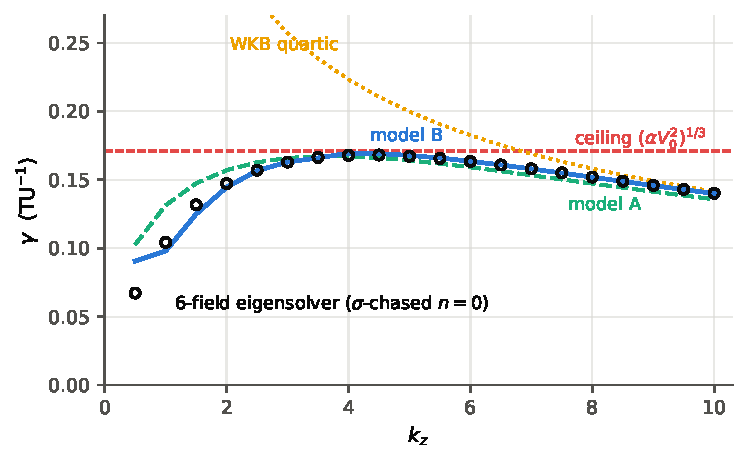
\includegraphics[width=0.74\textwidth]{fig_dispersion.pdf}
\caption{The full theory chain on one dispersion curve ($\alpha=2$,
$\Vo=0.05$, $\eps=0.15$, hard cut $\xi_w=11$; regenerated for this
document, no cached values). Open circles: dominant ($\sigma$-chased
$n=0$) eigenvalues of the six-field system \eqref{eq:sixfield} at
$N_x=384$. Solid: model B (\S\ref{ssec:modelB}) --- agreement
$\le0.2\%$ for $\kz\ge2.5$ here, degrading to a few percent only at
$\kz\lesssim1.5$ where the well is least square. Dashed: closed-form
model A \eqref{eq:modelA}. Dotted: the WKB quartic \eqref{eq:quartic},
overshooting at low $\kz$ exactly as diagnosed in \S\ref{sec:gap}. The
curve peaks at $\kz=4.5$ at $98\%$ of the ceiling (dashed red), and the
peak location matches eq.~\eqref{eq:kzpeak}: $0.1\times(11-\ln2)+3.42
=4.45$.}
\label{fig:dispersion}
\end{figure}

\subsection{Overtone ladder and eigenvalue-selection hygiene}
\label{ssec:ladder}

The action $S(\gamma)$ decreases as $\gamma$ increases (a faster-growing
mode has a shallower well: both $G-\gamma^2$ and $Q$ shrink,
\S\ref{ssec:resonance}), so the equation $S(\gamma)=\Phi+n\pi$ has one
root per $n$, forming a ladder $\gamma_0>\gamma_1>\dots$ --- the $n$-th
rung fitting $n$ extra half-waves into the well, as anticipated at the
top of the section --- with spacing
\begin{equation}
\Delta\gamma\simeq\frac{\pi}{|\partial S/\partial\gamma|},
\label{eq:ladderspacing}
\end{equation}
a few $\times10^{-2}\,$TU$^{-1}$ at loose windows: the rungs sit close
together. That spacing matters because of how large eigenvalue problems
are solved in practice. A library such as ARPACK does not return all
$6N$ eigenvalues of the discretized six-field system; it is handed a
target value $\sigma$ --- a guess at the answer --- and returns the
eigenvalue \emph{nearest that guess} (``shift-invert'' mode). If the
guess happens to land closer to rung $n=3$ than to rung $n=0$, the
solver hands back the overtone: correctly converged, numerically
impeccable, and silently the wrong mode. Exactly this happened. The
legacy default guess $\sigma=0.55\,\gamma_{\mathrm{WKB}}(\text{quartic})$
lands mid-ladder wherever the quartic underestimates (low $\alpha$, or
$\kz$ above the quartic's peak). Consequence (referee-critical,
discovered via this theory): at $(\alpha,\Vo,\kz)=(1,0.05,4)$, window
20, the dominant mode has $\gamma=0.134$ but default-$\sigma$ returned
$0.106$, and the cached survey curve carried $0.082$ --- an $n\approx3$
overtone; the eigenmode-seeded simulation then faithfully grew the
overtone it was seeded with ($0.081$, confirmed on a stable
fit-window plateau). \emph{Simulation-vs-solver agreement certifies
numerics, not dominant-mode selection.} All reference data now use
$\sigma$-chasing: re-solving with the target $\sigma$ shifted upward,
repeatedly, until no faster eigenvalue appears above the one found ---
i.e.\ until the returned mode is demonstrably the top rung $n=0$.
% ==============================================================================
\section{The dispersion curve: confinement-set peak and windowed roll-off}
\label{sec:peak}

\subsection{No intrinsic $\kz$ maximum}
\label{ssec:nopeak}

In an unbounded domain nothing stops the eigenmode from following the
resonance surface \eqref{eq:xires} outward as $\kz$ grows: the drive at
resonance is always $G_{\max}=\alpha\Vo^2/\gamma$, independent of $\kz$,
so $\gamma(\kz)$ rises monotonically and saturates at the ceiling
\eqref{eq:ceiling} while the mode migrates outward. Directly demonstrated
(eigensolver, $\alpha=2$, $\Vo=0.05$, cut $40$): $\gamma$ climbs to
$0.9955\,\Ceil$ by $\kz=10$ with no turnover, mode peak at $\xi=-36$. The
non-monotonic measured dispersion is therefore \emph{windowed physics},
not an intrinsic wavelength selection.

\subsection{The peak: resonance surface meets the window}
\label{ssec:kzpeak}

\begin{step}
For $\kz$ below the peak, the resonance surface
$\xi_{\mathrm{res}}(\kz)$ of \eqref{eq:xires} lies inside the window and
the mode enjoys the full resonant drive: $\gamma$ near the ceiling.
\end{step}

\begin{step}
Once $\xi_{\mathrm{res}}$ reaches the window radius $\xi_w$, the well is
truncated at the wall value of the covariant wavenumber,
$u_w=\alpha\Vo(\xi_w-\ln2)$, the resonance is no longer accessible, and
only the detuned drive $G(\kz)$ of \eqref{eq:GofK} remains: $\gamma$ rolls
off (next subsection). The peak is the crossover
$\xi_{\mathrm{res}}(\kz)=\xi_w$:
\begin{equation}
\frac{\kz-\gamma/\Vo}{\alpha\Vo}+\ln2=\xi_w .
\end{equation}
\end{step}

\begin{step}
At the crossover the mode still runs at essentially the ceiling, so
substitute $\gamma=\Ceil=(\alpha\Vo^2)^{1/3}$, i.e.
$\gamma/\Vo=(\alpha/\Vo)^{1/3}=\Kwn$:
\begin{equation}
\boxed{\;
\kz^{\mathrm{peak}}\simeq\alpha\Vo\,(\xi_w-\ln2)
+c\,\Bigl(\frac{\alpha}{\Vo}\Bigr)^{1/3},
\qquad c=1.0\pm0.1
\;}
\label{eq:kzpeak}
\end{equation}
($c$ absorbs the residual quantization offset; the empirical fit across
11 series gives $c$ in $0.85$--$1.0$). Both terms are \emph{independent of
$\eps$}: the shear width does not select the wavelength --- the coupling
and the containment radius select it together. Verified to $\pm0.6$ in
$\kz$ on all 11 usable series, including the direct window test: moving
the cut $11\to25$ at fixed physics ($\alpha=2$, $\Vo=0.05$) moved the
measured peak $4.5\to5.5$ (formula: $4.45\to5.85$). Both tests are shown
in Fig.~\ref{fig:peak}.
\end{step}

\begin{intuition}
The fence picks the wavelength. Every $\kz$ wants to sit on its own
resonance shell $\xi_{\mathrm{res}}(\kz)$, and the shells march outward
linearly with $\kz$. The window is a fence: modes whose shell is inside
run at essentially the ceiling; the first shell outside the fence marks
the peak; beyond it the mode is pinned at the wall with only the
detuned drive left, and rolls off. Nothing about the layer width $\eps$
enters --- for a Kelvin--Helmholtz-type instability this is the most
counter-intuitive single statement of the theory, and it is what the
data (peak drifting with window radius at fixed physics) confirmed
directly.
\end{intuition}

\begin{figure}[t]
\centering
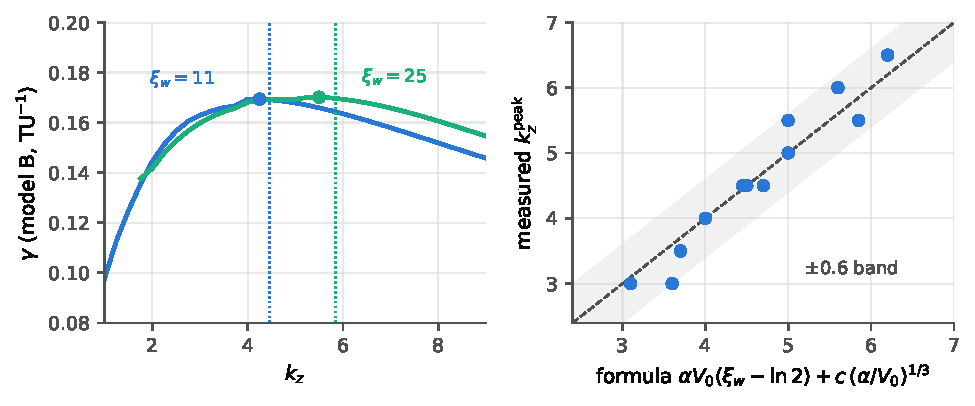
\includegraphics[width=\textwidth]{fig_peak.pdf}
\caption{The confinement-set peak. \emph{Left}: model-B dispersion
curves at fixed physics ($\alpha=2$, $\Vo=0.05$, $\eps=0.15$) for two
window radii: widening the cut $11\to25$ moves the peak (dots) from
$\kz\approx4.3$ to $\approx5.6$; dotted verticals are formula
\eqref{eq:kzpeak} with $c=1$. \emph{Right}: measured dominant-branch
peaks vs the formula across the validation series
($\alpha=1$--$5$, $\Vo=0.03$--$0.2$, $\xi_w=5$--$25$; the shaded band is
$\pm0.6$ in $\kz$).}
\label{fig:peak}
\end{figure}

\subsection{Beyond-peak roll-off}
\label{ssec:rolloff}

Past the peak, model A applies with the window-truncated well. Two limits
of \eqref{eq:modelA}:

\begin{step}[Loose-window limit $X\to0$]
$1+X^2\to1$ gives the envelope of the truncated branch,
\begin{equation}
\gamma^2=\tfrac12\Bigl[-\Vo^2\kz^2+\sqrt{\Vo^4\kz^4+8\alpha\Vo^3\kz}\Bigr].
\label{eq:rolloffexact}
\end{equation}
\end{step}

\begin{step}[High-$\kz$ asymptotics]
For $8\alpha/(\Vo\kz^3)\ll1$ expand the square root,
$\sqrt{1+\epsilon}\simeq1+\epsilon/2$ with
$\epsilon=8\alpha/(\Vo\kz^3)$:
\begin{equation}
\gamma^2\simeq\tfrac12\,\Vo^2\kz^2\cdot\frac{4\alpha}{\Vo\kz^3}
=\frac{2\alpha\Vo}{\kz}
\qquad\Longrightarrow\qquad
\boxed{\;\gamma\simeq\sqrt{\frac{2\alpha\Vo}{\kz}}\;}
\label{eq:rolloff}
\end{equation}
--- the measured beyond-peak decline ($\gamma\propto\kz^{-1/2}$),
steepened further by the $(1+X^2)^{-1}$ quantization factor as the
truncated well narrows.
\end{step}

\subsection{Why the data said $\kz^{\mathrm{peak}}\approx2\alpha$;
$\gamma^{\mathrm{peak}}$}
\label{ssec:2alpha}

Over the surveyed grid ($\alpha=1$--$5$, $\Vo=0.03$--$0.1$, window radii
shrinking as $\alpha$ grew, roughly $\alpha\Vo\xi_w\approx1$), formula
\eqref{eq:kzpeak} numerically tracks $\approx2\alpha$: the sub-linear
resonance term $(\alpha/\Vo)^{1/3}$ plus a window term whose radius the
campaign design shrank as $\alpha$ grew mimics a linear trend across a
factor-5 range of $\alpha$. The ``$\kz^{\mathrm{peak}}\approx2\alpha$
law'' is a serviceable survey-box mnemonic; \eqref{eq:kzpeak} is the law.
Similarly, the empirical $\gamma^{\mathrm{peak}}\sim\Vo^{0.85-0.92}$ at
fixed $\alpha$ is the ceiling's $\Vo^{2/3}$ times the window/quantization
correction $\hat\gamma(\text{budget},\alpha\Vo\xi_w)$, which increases
with $\Vo$ across the surveyed range;
$\gamma^{\mathrm{peak}}=(0.95$--$0.99)\,\Ceil$ for $\xi_w\ge8$, dropping
to ${\sim}0.95\,\Ceil$ at $\xi_w=5$.

% ==============================================================================
\section{Shear-width scaling: the quantization budget}
\label{sec:budget}

How does $\eps$ enter, given that neither the ceiling \eqref{eq:ceiling}
nor the peak formula \eqref{eq:kzpeak} contains it? Answer: only through
the \emph{action}, i.e.\ the quantization budget. We nondimensionalize the
exact action integral step by step. (This underlies the EPS-scan~v2
campaign design and its Phase-0 theory,
\texttt{analysis/eps\_collapse\_theory.py}.)

\begin{step}[Exact action in the $w$ variable]
In the saturated region, $u=\alpha\Vo(|\xi|-\ln2)$ and $x=\eps\,\xi$ give
$\dd x=\eps\,\dd\xi=\dfrac{\eps}{\alpha\Vo}\,\dd u$, and $w=\kz-u$ makes
$|\dd w|=|\dd u|$:
\begin{equation}
S=\int_{\mathrm{well}}\sqrt{Q}\,\dd x
=\frac{\eps}{\alpha\Vo}\int_{\mathrm{well}}\sqrt{Q}\,\dd w .
\end{equation}
\end{step}

\begin{step}[Hatted integrand]
With $w=\Kwn\hat w$ and \eqref{eq:Ghat},
\begin{align}
\D&=\gamma^2+\OmA\OmF=\gamma^2+w\,(2\kz-w)
=\Kwn^2\Bigl[\hat w\,(2\hat k-\hat w)+\Vo^2\hat\gamma^2\Bigr]
\equiv \Kwn^2\,\hat{\D},\\
Q&=\frac{\D\,(G-\gamma^2)}{\gamma^2}
=\Kwn^2\;\frac{\hat\D\,\bigl(\hat G-\hat\gamma^2\bigr)}{\hat\gamma^2}
\equiv\Kwn^2\,\hat Q(\hat w;\hat k,\hat\gamma)
\end{align}
(the factors $\Ceil^2$ from $G-\gamma^2$ and $\gamma^2$ cancel; the
explicit $\Vo^2\hat\gamma^2\le0.04$ inside $\hat\D$ is negligible over the
production range, so $\hat Q$ is universal in hatted variables).
\end{step}

\begin{step}[Assembled scaling]
Using $\dd w=\Kwn\,\dd\hat w$ together with
\begin{equation}
\frac{\Kwn^2}{\alpha\Vo}
=\Bigl(\frac{\alpha}{\Vo}\Bigr)^{2/3}\frac{1}{\alpha\Vo}
=\alpha^{-1/3}\Vo^{-5/3}
=\frac{1}{\Vo\,(\alpha\Vo^2)^{1/3}},
\end{equation}
we obtain
\begin{equation}
\boxed{\;
S=\frac{\eps\,\Kwn^2}{\alpha\Vo}\int\sqrt{\hat Q}\,\dd\hat w
=\frac{\eps}{\Vo\,(\alpha\Vo^2)^{1/3}}\;\hat I(\hat k,\hat\gamma),
\qquad
\hat I\equiv\int_{\hat w\text{-well}}\sqrt{\hat Q}\,\dd\hat w
\;}
\label{eq:budget}
\end{equation}
(numerically verified: at $\alpha=2$, $\Vo=0.05$, $\eps=0.15$, $\kz=4$,
$\gamma=0.16$, both sides give $S\approx2.8$ before quantization pulls
$\gamma$ up). The shear width therefore enters the eigenvalue problem
\emph{only} as a multiplicative budget on the action; the well's shape in
$\hat w$ is $\eps$-free.
\end{step}

\begin{remark}[Normalization of the program's ``$P$'' group]
The project's shorthand (PHYSICS.md eq.~(11.5)) writes
$S=(\eps/\Ceil)\int\sqrt{\hat Q'}\,\dd\hat w$ with the group
$P=\Ceil/\eps$; comparing with \eqref{eq:budget}, that convention absorbs
a factor $\Vo^{-2}$ into its $\hat Q'$ ($\hat Q'=\hat Q/\Vo^2$). The clean
statement is \eqref{eq:budget}: the dimensionless budget prefactor is
$\eps^{-1}\Vo(\alpha\Vo^2)^{1/3}=(\alpha\Vo^5)^{1/3}/\eps$, with the
integral $\hat I$ universal. Either bookkeeping gives identical model-A/B
numbers (the campaign tooling evaluates the models directly and never uses
the shorthand); the distinction matters only if one collapses \emph{data}
against a single ``budget group'', where the residual $\Vo$-dependence is
part of why a pure one-group collapse in
$P=(\alpha\Vo^2)^{1/3}/\eps$ is imperfect (cf.\ the observed
$\eps$-drift of $\kz^{\mathrm{peak}}$ at fixed window).
\end{remark}

\begin{remark}[Qualitative consequences]
Larger $\eps$ (at fixed window and physics) enlarges $S$ at given
$\gamma$, and since $S$ decreases in $\gamma$, quantization then pushes
$\gamma$ \emph{up} toward the ceiling --- the sign of the measured
$10$--$39\%$ rise of $\gamma$ from $\eps=0.10\to0.45$ at fixed
$(\kz,\xi_{\mathrm{sponge}})$; Fig.~\ref{fig:budget} shows the model-B
version of this rise. Because the budget also shifts which $\kz$
first saturates its quantization, $\kz^{\mathrm{peak}}$ acquires a mild
$\eps$-dependence even though \eqref{eq:kzpeak}'s leading terms have none.
\end{remark}

\begin{intuition}
$\eps$ buys action. Stretching the layer stretches the well in physical
$x$ while leaving its depth and shape unchanged in the scaled variable
$\hat w$ --- so at fixed $\gamma$ the mode accumulates more phase, and
the connection condition then lets $\gamma$ float up toward the ceiling.
The shear width is a \emph{budget} knob (how much quantization tax the
mode pays), not a wavelength selector; that is why its effect shows up
as a fractional rise of $\gamma$ everywhere rather than as a shift of
the physics scales $\Ceil$, $\Kwn$.
\end{intuition}

\begin{figure}[t]
\centering
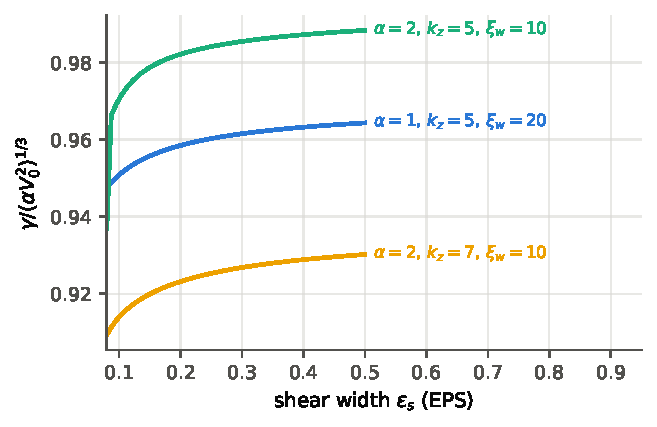
\includegraphics[width=0.58\textwidth]{fig_budget.pdf}
\caption{The quantization budget at work (model B, beyond-peak
window-limited points): at fixed physics and window, increasing the
shear width $\eps$ raises $\gamma$ toward the ceiling, exactly as
eq.~\eqref{eq:budget} prescribes --- $\eps$ enters only as a
multiplier on the action.}
\label{fig:budget}
\end{figure}

% ==============================================================================
\section{Diagnosis of the WKB quartic's domain of validity}
\label{sec:gap}

The quartic \eqref{eq:quartic} models the drive as the constant
$-\alpha^2\Vo\kz/\omega^2$ term of \eqref{eq:wkbQ0} --- one power of $v$
(from the current), one resonance-free factor $\alpha^2\Vo\kz$. The true
drive \eqref{eq:Gdef} has three powers of $v$, is Doppler-resonant, and is
ceiling-bounded by \eqref{eq:Gmax}. Comparing the two fixes exactly where
eq.~\eqref{eq:eq33}/\eqref{eq:quartic} can and cannot work:
\begin{itemize}
\item \textbf{Low $\kz$ (below the true peak):} the quartic's drive
$\alpha^2\Vo\kz/\gamma^2$ has no ceiling; as $\gamma$ is iterated it can
supply arbitrarily large growth, and the quartic overshoots the true
branch by the measured $10$--$20\times$ in the $\kz\lesssim1$ tail.
\item \textbf{High $\kz$:} the quartic's balance
$\omega^4-\kz^2\omega^2\approx\alpha^2\Vo\kz$ makes
$\gamma^2\approx\alpha^2\Vo/\kz$, a \emph{decline}, while the true
unbounded branch saturates at the ceiling; in windowed data the truncated
true branch declines as \eqref{eq:rolloff} instead. In the weak-coupling
corner this produces the observed ${\sim}25\%$ quartic underestimates.
\item \textbf{$\kz=0$:} the geometry changes (parabolic potential exact,
different channel); the harmonic-core quantization is exact there and the
$0.5\%$ chromo-Weibel anchor \eqref{eq:weibel} stands untouched by this
critique.
\end{itemize}
The quartic is thus a valid \emph{harmonic-core} theory (its own regime:
$\kz=0$ and the immediate neighborhood of a parabolic well) but not a
theory of the finite-$\kz$ shear branch; models A/B replace it there.

% ==============================================================================
\section{Cold two-stream rates in code units}
\label{sec:twostream}

The counter-streaming beams support, away from the shear layer
($v_z\to\pm\Vo$), an electrostatic color-1 two-stream instability. Its
exact cold rates in code units calibrate the bandpass-filter design
(Appendix~\ref{app:filters}) and were used to test (and reject) the
outer two-stream as the late-catastrophe driver.

\subsection{Dispersion relation}

\begin{step}
Longitudinal channel: perturbations $\propto e^{\ii(kz-\omega t)}$ of
$n_s$, $v_{zs}$, coupled by the longitudinal field $E_z$. Linearized
continuity and momentum for beam $s$ with background velocity $u_s$
(here $u_{A,B}=\pm V$), per-beam plasma frequency
\eqref{eq:omegap}:
\begin{equation}
\delta n_s=\frac{k\,n_0\,\delta v_s}{\omega-k u_s},\qquad
\delta v_s=\frac{\ii\,q_s E_z/m}{-(\ii)(\omega-ku_s)}
\;\Longrightarrow\;
\delta n_s=-\frac{n_0q_sE_z\,k/m}{(\omega-ku_s)^2}\cdot\frac1{\ii}\cdot\ii
=-\frac{kq_sn_0E_z/m}{(\omega-ku_s)^2}.
\end{equation}
\end{step}

\begin{step}
Poisson/Gauss ($\varepsilon_0=1$): $\ii kE_z=\sum_sq_s\delta n_s$ gives
\begin{equation}
\ii kE_z=-\sum_s\frac{kq_s^2n_0E_z/m}{(\omega-ku_s)^2}\cdot\frac1{\ii^{-1}}
\quad\Longrightarrow\quad
1=\sum_s\frac{\omega_{p}^2}{(\omega-ku_s)^2}
=\frac{1}{(\omega-kV)^2}+\frac{1}{(\omega+kV)^2}.
\label{eq:tsdisp}
\end{equation}
(the standard two-beam form; each beam contributes $\omega_p^2=1$).
\end{step}

\subsection{Closed-form growth rate}

\begin{step}[Reduce to a quadratic]
Put the right side of \eqref{eq:tsdisp} over a common denominator, using
$(\omega\mp kV)^2$ sum $=2(\omega^2+k^2V^2)$:
\begin{equation}
(\omega^2-k^2V^2)^2=2\,(\omega^2+k^2V^2).
\end{equation}
Let $y=\omega^2$ and $\beta=k^2V^2$:
\begin{equation}
(y-\beta)^2=2(y+\beta)
\quad\Longleftrightarrow\quad
y^2-2(\beta+1)\,y+\beta^2-2\beta=0 .
\end{equation}
\end{step}

\begin{step}[Solve]
\begin{equation}
y_\pm=(\beta+1)\pm\sqrt{(\beta+1)^2-\beta^2+2\beta}
=(\beta+1)\pm\sqrt{4\beta+1}.
\end{equation}
\end{step}

\begin{step}[Instability condition]
$y_-<0$ (i.e.\ $\omega^2<0$, purely growing) iff
$(\beta+1)^2<4\beta+1$ iff $\beta^2<2\beta$ iff $\beta<2$:
\begin{equation}
\boxed{\;kV<\sqrt2\;}
\qquad\text{unstable band.}
\label{eq:tsband}
\end{equation}
At $\Vo=0.1$ this is $k<14.1$ --- exactly the documented
$k_{\mathrm{ts}}\approx14$ two-stream band that fixed the production
bandpass edge.
\end{step}

\begin{step}[Growth rate, maximum, small-$k$ limit]
\begin{equation}
\boxed{\;
\gamma^2(kV)=-y_-=\sqrt{4(kV)^2+1}-(kV)^2-1
\;}
\label{eq:tsgamma}
\end{equation}
Maximize over $\beta$: $\dd\gamma^2/\dd\beta=2/\sqrt{4\beta+1}-1=0$ gives
$\beta=3/4$, i.e.\
\begin{equation}
kV=\frac{\sqrt3}{2},\qquad
\gamma_{\max}^2=\sqrt{4}-\tfrac34-1=\tfrac14,\qquad
\gamma_{\max}=\tfrac12 .
\end{equation}
Small $kV$: $\sqrt{4\beta+1}\simeq1+2\beta-2\beta^2$ gives
$\gamma^2\simeq\beta$, i.e.\ $\gamma\simeq kV$. (Measured full-domain
rates $0.7$--$0.9$ exceed $\tfrac12$ because they include the
electromagnetic/Weibel corrections outside this electrostatic model.)
The full curve is Fig.~\ref{fig:twostream}.
\end{step}

\begin{intuition}
Bunching in a moving mirror. In the frame of one beam, the other beam's
charge bunches stream past and their electric field does work on the
first beam's particles, bunching them in turn; below the band edge the
bunches of each beam arrive in phase with the wells of the other and the
loop closes. The band edge $kV=\sqrt2$ is where the streaming Doppler
shift finally outruns the plasma response. In code units
($\omega_p=1$ per beam) the band at $\Vo=0.1$ ends at $\kz=14.1$ ---
the number that fixed the production bandpass-filter edge, and the
theory whose \emph{spatial} predictions (growth localized in the outer
$|v_z|\approx\Vo$ region) were used to rule the two-stream out as the
late-catastrophe driver.
\end{intuition}

\begin{figure}[t]
\centering
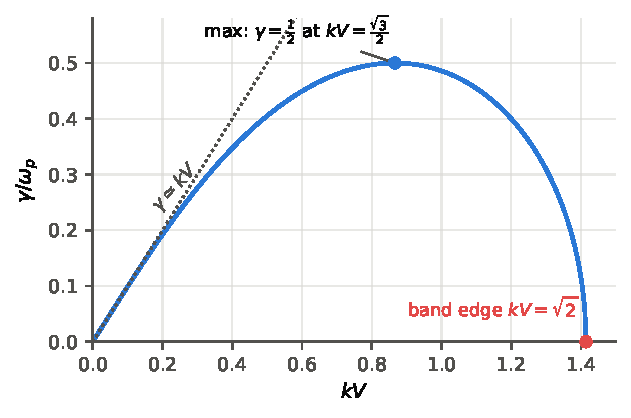
\includegraphics[width=0.55\textwidth]{fig_twostream.pdf}
\caption{Exact cold two-stream growth rate \eqref{eq:tsgamma} in code
units: $\gamma\simeq kV$ at long wavelength, maximum $\gamma=\tfrac12$
at $kV=\sqrt3/2$, band edge at $kV=\sqrt2$
(eq.~\eqref{eq:tsband}).}
\label{fig:twostream}
\end{figure}

% ==============================================================================
\section{Nonlinear theory: cavitation threshold and the back-reaction law}
\label{sec:nonlinear}

\subsection{Density cavitation of the finite-amplitude KH mode}
\label{ssec:cavitation}

The linear eigensolver state vector contains no fluid density/momentum
blocks; the late-time ``hard wall'' at $\Vo\gtrsim0.08$ is a nonlinear
fluid effect. Its threshold is derived as follows.

\begin{step}[First-order compressive response]
Linearize \eqref{eq:continuity} about $n=1$ for a mode
$\propto e^{\gamma t}$:
\begin{equation}
\gamma\,\delta n=-\bigl(\ii\kz\,\delta p_z+\partial_x\,\delta p_x\bigr)
\qquad\Longrightarrow\qquad
|\delta n|\sim\frac{\kz\,|p_{z1}|+k_x^{\mathrm{eff}}\,|p_{x1}|}{\gamma},
\end{equation}
where $k_x^{\mathrm{eff}}$ is the mode's inverse $x$-scale.
\end{step}

\begin{step}[Second-order (ponderomotive) part]
Quadratic beats of the mode grow at $2\gamma$ and accumulate a $z$-mean
density modification; the observed density-perturbation growth at the
retained $\kz$ at twice the saturating field rate is this quadratic part
taking over as the fields saturate.
\end{step}

\begin{step}[Cavitation threshold]
Cavitation ($\delta n\to n_0$, i.e.\ $n$ hits the code floor $0.05$)
occurs when the momentum amplitude reaches
\begin{equation}
\boxed{\;p_{\mathrm{cav}}\sim\frac{\gamma}{\max(\kz,\,k_x^{\mathrm{eff}})}\;}
\label{eq:pcav}
\end{equation}
(order of magnitude). Beyond it, the floored divisions
$v=p/\max(n,0.05)$ decouple momentum from density and the model no longer
represents the physical system; a long-lived floored-pocket state persists
for tens of TU before terminal blow-up. Because \eqref{eq:pcav} is an
\emph{amplitude} threshold, whether a run cavitates within its length is
controlled by drive strength ($\Vo$, through $\gamma$ and the saturation
level) and effective seed --- hence the observed gradual
$\Vo=0.05\to0.10$ transition, its insensitivity to window mechanism and
radius, and the practical rule of capping \texttt{target\_tu} just past
the plateau at high $\Vo$. Forensics on a failing run localized every
growing channel at the shear layer ($99.9\%$ of density-perturbation
power at $|\xi|<5$) with the outer region quiet, ruling out the outer
branches as the driver.
\end{step}

\begin{intuition}
The mode digs its own grave. A growing wave in a compressible fluid
carries a density modulation proportional to its momentum amplitude over
$\gamma$; on top of it, the quadratic (ponderomotive) beat pushes plasma
out of the high-field regions at rate $2\gamma$. When the excavated
fraction reaches the background density, the fluid description --- and
the code's floored version of it --- stops representing the plasma.
The threshold \eqref{eq:pcav} is an \emph{amplitude} cliff, not a time
cliff: that single fact explains why the failure zone maps onto drive
strength ($\Vo$), why it cares little about window design, and why the
only safe practice at high $\Vo$ is to stop measuring once the linear
plateau is banked.
\end{intuition}

\subsection{Structure of the back-reaction on $\Az$: the quadratic law}
\label{ssec:backreaction}

Unfreezing $A_z^1$ lets the color-2/3 wave imprint on the background. The
measured law (two independent configurations, four decades of $|a|^2$,
endpoint exact) is
\begin{equation}
\Delta\Az\simeq-0.04\,|a|^2 ,
\label{eq:dazlaw}
\end{equation}
localized at the mode peak, i.e.\ the wave \emph{deepens} $|\Az|$ ---
opposite in sign to depletion. The structure (quadratic, $\kz=0$,
localized, growing at $2\gamma$) is derived as follows; the coefficient
and sign are taken from measurement.

\begin{step}[All color-1 second-order sources are helicity beats]
For real fields with circular structure
$X^2=\Rey(\hat Xe^{\ii\kz z})$, $X^3=\Imy(\hat Xe^{\ii\kz z})$, any
color-1 cross-product source is a beat of two color-2/3 waves, e.g.\ for
the precession of $Q^1$:
\begin{equation}
(\vec Q\times\vec A_z)^1=Q^2A_z^3-Q^3A_z^2
=\Rey(\hat qe^{\ii\theta})\,\Imy(\hat ae^{\ii\theta})
-\Imy(\hat qe^{\ii\theta})\,\Rey(\hat ae^{\ii\theta})
=\Imy\bigl(\hat a\,\hat q^{\,*}\bigr),
\qquad \theta=\kz z ,
\label{eq:beat}
\end{equation}
which is \emph{independent of $z$}: the color-1 imprint of a circular
mode is purely $\kz=0$, and $\propto|{\rm amplitudes}|^2\,e^{2\gamma t}$.
The same computation applies to the current beats
($\delta n\,\delta v_z$, $\delta Q^{2,3}\,\delta v_z$ contributions to
$J_z^1$) and to the field commutator beats in
\eqref{eq:amperex}/\eqref{eq:faraday}.
\end{step}

\begin{step}[Chain to $\Delta\Az$]
The $\kz=0$ color-1 source drives $J_z^1{}^{(2)}\to E_z^1$ (Amp\`ere-$z$),
and $\partial_t\Az=-E_z^1$ integrates it. With every second-order source
$\propto e^{2\gamma t}$, each time integration divides by $2\gamma$, so
\begin{equation}
\Delta\Az(t)=-\frac{\text{(source strength)}}{(2\gamma)^2}\,
e^{2\gamma t}\;\propto\;-\,|a(t)|^2 ,
\end{equation}
a pure quadratic law in the instantaneous mode amplitude, pinned at the
mode peak --- exactly the measured structure \eqref{eq:dazlaw}
(Fig.~\ref{fig:backreaction}).
\end{step}

\begin{figure}[t]
\centering
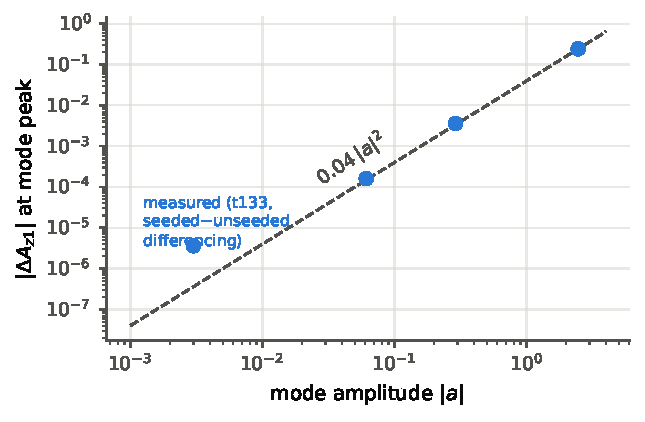
\includegraphics[width=0.52\textwidth]{fig_backreaction.pdf}
\caption{The measured back-reaction law against the derived quadratic
structure: $|\Delta\Az|$ at the mode peak vs the instantaneous mode
amplitude $|a|$, from seeded-minus-unseeded differencing of unfrozen
runs (t133; two configurations pooled). The dashed line is
$0.04\,|a|^2$: slope $2$ over four decades, endpoint exact
($-0.242$ vs $-0.242$ at $|a|=2.46$). The \emph{sign} deepens the
background --- no depletion.}
\label{fig:backreaction}
\end{figure}

\begin{intuition}
Waves weigh on their background. Any quadratic beat of a
single-helicity mode is $z$-independent (eq.~\eqref{eq:beat}) --- a DC
force growing at $2\gamma$ --- so the wave exerts a steady,
locally-confined push on the color-1 sector wherever its envelope
peaks, like radiation pressure. Here the push happens to point
``downhill'': it makes $|\Az|$ larger, recharging rather than draining
the battery. That closes the last escape route for the frozen-background
caveat: even fully self-consistent, the tachyonic branch does not switch
itself off by depletion; the model's true nonlinear endpoint is the
fluid one (\S\ref{ssec:cavitation}).
\end{intuition}

\begin{step}[Consequences]
Since $\Delta\Az<0$ where $\Az<0$, $|\alpha\Az|$ grows: no depletion of
the battery. The clean frozen/unfrozen pair shows the global effect is
weakly stabilizing (mode amplitude $-7\%$ by $|a|\approx2.5$; annulus
compression against the fixed damping boundary), two orders of magnitude
too weak to saturate the branch: saturation is by fluid nonlinearity
(\S\ref{ssec:cavitation}), not background drain, and the frozen-$\Az$
approximation is accurate to a few percent everywhere it matters
(validated: unfrozen linear rate unchanged, $\gamma=1.45$ vs eigensolver
$1.43$--$1.46$ at the reference blow-up).
\end{step}

% ==============================================================================
\section{Warm isothermal fluid closure}
\label{sec:warm}

\subsection{Derivation of the pressure source}

Take the first velocity moment of the kinetic equation for beam $s$ with
an isotropic thermal spread $T$ (code units, $m=1$):
\begin{equation}
\partial_t p_i+\partial_j\bigl(v_jp_i\bigr)
=-\partial_i P+F_i,
\qquad P=nT\quad(\text{isothermal closure}),
\end{equation}
so the only new term relative to the cold model
\eqref{eq:momx}--\eqref{eq:momz} is the momentum-density source
\begin{equation}
\boxed{\;\delta F_i=-T\,\partial_i n\;}
\end{equation}
(no extra $1/n$: the sources are momentum-density rates). $T=0$ recovers
the cold system identically. Linearly, the closure adds the sound term
$c_s^2=T$ to the fluid response: the two-stream channel of
\S\ref{sec:twostream} acquires the standard thermal stabilization when
$v_{\mathrm{th}}=\sqrt T\gtrsim\Vo$ (Landau-fluid analogue of
$kV<\sqrt2\,\omega_p$ shrinking), which was the intended validation
target.

\subsection{Why it cannot stabilize the $\kz=0$ chromo-Weibel}

The $\kz=0$ mode of \S\ref{ssec:weibel} is a filamentation
(Weibel-class) instability driven by the momentum-space
\emph{anisotropy} of the counter-streaming beams. An isotropic scalar
pressure $P=nT$ adds a restoring force only along density gradients of
the compressive response; it does not relax the anisotropy that powers
filament growth. The scan confirmed this: across
$v_{\mathrm{th}}/\Vo=0$--$3$ the final $\kz=0$ amplitude changed by only
${\sim}11\%$. (The clean warm-vs-cold validation was subsequently obtained
on the KH target point itself: with the corrected control, warm-closure
rates match the cold theory at the $1\%$ level, closing T1.4.)

% ==============================================================================
\section{Eigenmode seeding theory}
\label{sec:seeding}

\subsection{Hermite ground state of the harmonic core}
\label{ssec:hermite}

The harmonic core of the given theory,
$\partial_x^2a+(Q_0-|C_1|x^2)a=0$ (from \eqref{eq:wkbQ}), is exactly the
quantum harmonic oscillator: with $\sigma\equiv|C_1|^{-1/4}$,
eigenfunctions and eigenvalues are
\begin{equation}
a_n(x)=H_n\!\Bigl(\frac{x}{\sigma}\Bigr)\,
e^{-x^2/2\sigma^2},
\qquad
Q_0=(2n+1)\sqrt{|C_1|},
\end{equation}
i.e.\ eq.~\eqref{eq:eq33} \emph{is} the oscillator spectrum, and the
$n=0$ eigenfunction is the Gaussian
\begin{equation}
\boxed{\;
a_0(x)=\exp\Bigl(-\frac{x^2}{2\,\xi_{\mathrm{char}}^2}\Bigr),
\qquad
\xi_{\mathrm{char}}=|C_1|^{-1/4}
=\Bigl(\frac{2\,\gamma^2}{\alpha^3\Vo^2}\Bigr)^{1/4}
\;}
\label{eq:xichar}
\end{equation}
(using $|C_1|=\alpha^3\Vo^2/(2\omega^2)$, $\omega^2\to-\gamma^2$ with the
magnitude convention of \S\ref{ssec:clearing}; $x$ here is the
$\xi$-coordinate of the step-potential form). With the high-$\kz$ quartic
balance $\gamma^2\approx\alpha^2\Vo/\kz$ (\S\ref{sec:gap}),
\begin{equation}
|C_1|\approx\frac{\alpha\Vo\kz}{2}
\qquad\Longrightarrow\qquad
\xi_{\mathrm{char}}\approx\Bigl(\frac{2}{\alpha\Vo\kz}\Bigr)^{1/4}.
\label{eq:xicharhighk}
\end{equation}

\begin{remark}[The implemented width]
Campaign 18's init kernel uses the simpler
$\xi_{\mathrm{char}}^{\mathrm{code}}=(\alpha\kz\Vo)^{-1/2}$, which
coincides with \eqref{eq:xicharhighk} exactly at $\alpha\Vo\kz=\tfrac12$
(both give $\sqrt2$) and tracks it within a few tens of percent over the
campaign grid $\alpha\Vo\kz\approx0.1$--$1.2$ (e.g.\ $\alpha=2$,
$\Vo=0.1$, $\kz=2$: code $1.58$ vs Hermite $\approx1.50$); the two have
different scaling exponents ($-1/2$ vs $-1/4$), visible in
Fig.~\ref{fig:seed}. A width mismatch only launches a transient that
decays within a few growth times, so the approximation is operationally
adequate; the exact profile is superseded anyway by full six-field
seeding (below).
\end{remark}

\begin{figure}[t]
\centering
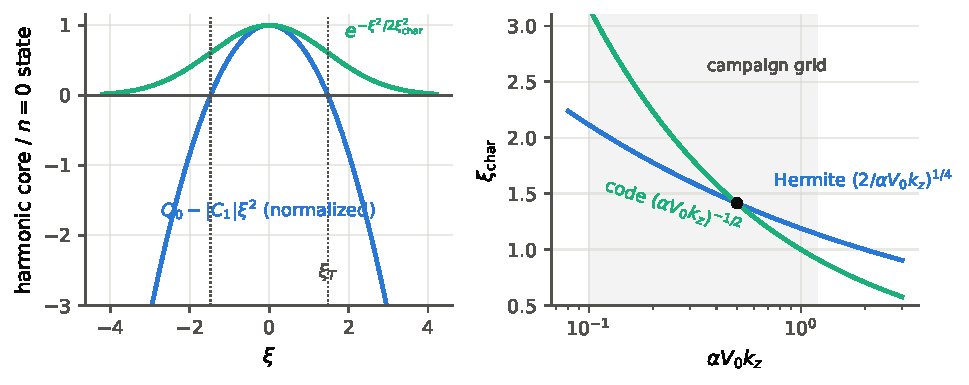
\includegraphics[width=\textwidth]{fig_seed.pdf}
\caption{Seeding theory. \emph{Left}: the harmonic core of the given
theory with its $n=0$ Hermite ground state \eqref{eq:xichar}
($\alpha=2$, $\Vo=0.1$, $\kz=2$; $\xi_T$ marks the harmonic turning
points): eq.~(33) of \texttt{wkb.pdf} \emph{is} the oscillator spectrum
and the natural seed is this Gaussian. \emph{Right}: the exact Hermite
width vs the implemented approximation $(\alpha\Vo\kz)^{-1/2}$: equal at
$\alpha\Vo\kz=\tfrac12$, within a few tens of percent over the campaign
grid (shaded), but with different power laws outside it.}
\label{fig:seed}
\end{figure}

\subsection{Why single-field seeding selects wrong modes}

An $A_z$-only (or $B_y$-only) seed fixes one field's profile and lets the
activation chain build the others; the projection of that initial
condition onto the eigenmode basis decides what grows first. Concretely
(C23): for the target mode at $(\alpha,\Vo,\kz)=(1,0.05,2)$ the $B_y$ and
$A_z$ profiles peak at different $\xi$ ($1.64$ vs $7.85$); an $A_z$-only
Gaussian placed correct-for-$A_z$ deposits the charge response at the
wrong location, and a different (co-located, slower) eigenmode wins the
race: measured $\gamma=0.060$ vs target $0.122$. The remedy is seeding
all six fields with the solver eigenvector (exact amplitude ratios and
phases), which removes the transient entirely; conversely
\S\ref{ssec:ladder} shows the seed must come from the \emph{dominant}
($\sigma$-chased) eigenvector, or the run will faithfully measure an
overtone.

\subsection{Cascade race condition}

Single-field $B_y$ seeding at $\kz\ge2$ loses a second race: the
layer-scale color mixing of \S\ref{ssec:tachyon} builds $A_z^{2,3}$ at
$\gamma_{\mathrm{casc}}\approx\alpha\Vo$ from any residual field, so if
$\gamma_{\mathrm{KH}}<\gamma_{\mathrm{casc}}$ the seed decays into the
cascade background before the KH chain closes. Gaussian $A_z$ seeding
(mode 6) pre-loads the slowest link of the chain
$a\to q_A\to$ Lorentz $\to b$ at the correct width
\eqref{eq:xichar}, which is why it (and its six-field successor) restored
clean linear windows at $\kz\ge2$.

\begin{intuition}
Seeding is choosing the initial overlap. A linear run does not measure
``the'' growth rate of the system --- it measures the growth rate of
whatever eigenmode dominates the projection of its initial condition
once transients die. Every seeding pathology of the program is this one
sentence in different clothes: the C23 stray mode (an $A_z$-only seed
overlapping a co-located slower mode better than the target), the
cascade race (a $B_y$ seed whose target projection decays before the
chain closes), and the overtone trap of \S\ref{ssec:ladder} (a perfect
six-field seed of the \emph{wrong rung}, faithfully grown by a perfect
simulation). The cure in every case is the same: know the spectrum
first, then seed the intended member of it.
\end{intuition}

\clearpage
\appendix

% ==============================================================================
\section{Helicity projections and the conjugate-extraction identity}
\label{app:helicity}

For a circular mode the two real fields are
\begin{equation}
A_z^2(x,z)=\Rey\bigl[\hat a(x)e^{\ii\kz z}\bigr],\qquad
A_z^3(x,z)=\Imy\bigl[\hat a(x)e^{\ii\kz z}\bigr],
\end{equation}
so the complex pair is single-signed in $\kz$:
$a=A_z^2+\ii A_z^3=\hat a(x)\,e^{\ii\kz z}$ exactly. Its $z$-DFT
therefore has \emph{all} its weight at $+\kz$ and none at $-\kz$:
\begin{equation}
\tilde a(+\kz)=\hat a,\qquad \tilde a(-\kz)=0 .
\label{eq:helproj}
\end{equation}
Writing the projections in real arithmetic with $c=\cos\kz z$,
$s=\sin\kz z$:
\begin{equation}
\tilde a(\pm\kz)\propto\sum_z\bigl[(A_z^2c\pm A_z^3s)
+\ii\,(\mp A_z^2s+A_z^3c)\bigr].
\end{equation}
The extraction bug of 2026-07-04$\to$07-17 computed the lower sign (the
$-\kz$, conjugate-helicity projection): by \eqref{eq:helproj} this is
\emph{identically zero} for a pure circular mode, and what it actually
returned on real data was the small opposite-helicity contamination ---
hence amplitudes at the $e^{-25}$ floor and the triage rule
``first-amplitude $<e^{-25}$ $\Rightarrow$ invalid extraction''. The
mirror symmetry of \S\ref{ssec:helicity} guarantees the physical
information lives in one helicity per side of the layer, so the corrected
single-sign projection loses nothing.

% ==============================================================================
\section{Filters, sponges, and hyperdiffusion as linear operators}
\label{app:filters}

\paragraph{DFT band filter.} \texttt{kernel\_ym\_subtract\_kz\_range}
applies, each step, the projection
$f\mapsto f-\sum_{k\in\mathcal B}\Pi_kf$, where $\Pi_k$ is the exact DFT
projector onto $z$-mode $k$ and $\mathcal B=\{1,\dots,k_{\mathrm{lo}}\}
\cup\{k_{\mathrm{mode}}+1,\dots,k_{\mathrm{hi}}\}$: an idempotent linear
operator that removes the two-stream band \eqref{eq:tsband} while leaving
the measured mode untouched. The same projector acts on the fluid
$p_z$'s. (Empirical constraint, recorded not derived: keep
$k_{\mathrm{hi}}\le N_Z/4.5$ so the projector's stencil does not interact
with the FCT limiter's near-Nyquist deposits.)

\paragraph{Sponge.} \texttt{kernel\_ym\_sponge} adds
$\partial_tf=-\sigma_s(\xi)f$ with
$\sigma_s=\sigma\,(|\xi|-\xi_{\mathrm{sponge}})_+$: a non-Hermitian
absorbing potential. In the eigenproblem it appears as
$-\sigma_s(\xi)$ on the diagonal of all blocks; it removes the outer
branch of \S\ref{ssec:tachyon} when $\xi_{\mathrm{sponge}}
<\xi_{\mathrm{crit}}$ (legitimate, by the battery argument) at the cost
of the few-percent well compression measured in the sponge-vs-cut
comparisons.

\paragraph{Hard cut.} \texttt{xi\_cut} zeroes all wave fields outside
$\xi_w$: Dirichlet/Neumann wall pair of \S\ref{ssec:discrete}.

\paragraph{Hyperdiffusion.} The $z$-hyperdiffusion adds
$\partial_tf=-\mu\,\partial_z^4f$, i.e.\ damping $\mu k^4$ per mode: with
$\mu=5\times10^{-5}$ it removes grid-scale noise while its drag on a
retained mode $k$ is $\mu k^4\ll\gamma$ for all production $k$ (e.g.\
$k=6$: $\mu k^4=0.065\gamma$ at $\gamma=0.1$; the design condition is
$1/(\mu k^4)\gg1/\gamma$).

% ==============================================================================
\section{Validation ledger}
\label{app:ledger}

\begin{center}
\begin{tabular}{p{0.52\textwidth}p{0.40\textwidth}}
\toprule
\textbf{Derived result} & \textbf{Numerical anchor}\\
\midrule
Quartic $\kz{=}0$ chromo-Weibel rate \eqref{eq:weibel} &
sim vs formula: $0.5\%$; $\gamma=0.284$ reproduced at the $\alpha=1$,
$\Vo=0.05$ reference\\[2pt]
Six-field system \eqref{eq:sixfield} &
eigensolver vs 2D CUDA growth rates: $1$--$4\%$ (plateau-confirmed clean
cores: median $6$--$10\%$ archive-wide)\\[2pt]
Exact reduction \eqref{eq:reduced}/\eqref{eq:discretereduced} &
reduced operator vs 6-field ARPACK: rel.\ diff.\ $0.0$ ($<10^{-10}$) at 7
points, $\alpha=1$--$3$, $\Vo=0.03$--$0.1$, $\kz=1$--$7$\\[2pt]
Tachyonic law \eqref{eq:gloc}--\eqref{eq:xicrit} &
analytic envelope $=$ float64 eigensolver $=$ float32 CUDA rates at all
outer eigenmode peaks; blow-up $\gamma=1.45$ vs $1.43$--$1.46$\\[2pt]
Ceiling \eqref{eq:ceiling} &
dominant-branch peaks at $95$--$99\%$ of $(\alpha\Vo^2)^{1/3}$ in every
series; T2.5 collapse $\gamma_{\mathrm{peak}}/\Ceil=0.977\pm0.011$\\[2pt]
Model B quantization (\S\ref{ssec:modelB}) &
$\le2\%$ (median $\le0.2\%$) vs $\sigma$-chased $n{=}0$ eigenvalues,
12 series, $\kz\ge1.5$\\[2pt]
Model A closed form \eqref{eq:modelA} &
${\sim}3\%$ near/above peak; peak located to $\pm0.5$ in $\kz$\\[2pt]
Peak formula \eqref{eq:kzpeak} &
$\pm0.6$ in $\kz$ across 11 series; window test: cut $11\to25$ moved peak
$4.5\to5.5$ (formula $4.45\to5.85$)\\[2pt]
Two-stream band \eqref{eq:tsband} &
$k_{\mathrm{ts}}\approx14$ at $\Vo=0.1$ (documented band edge)\\[2pt]
Back-reaction law \eqref{eq:dazlaw} &
$\Delta\Az=-0.04|a|^2$ over four decades; endpoint $-0.242$ vs $-0.242$\\[2pt]
Warm closure (\S\ref{sec:warm}) &
warm vs cold theory at the KH target: $1\%$ (corrected control)\\
\bottomrule
\end{tabular}
\end{center}

\end{document}
